\documentclass[10pt,a4paper]{article}
\usepackage[a4paper,margin=17mm]{geometry}
\usepackage[T1]{fontenc}
\usepackage{lmodern}
\usepackage{amsmath,amssymb}
\usepackage{graphicx}
\usepackage{booktabs}
\usepackage{array}
\usepackage{caption}
\usepackage{subcaption}
\usepackage{tikz}
\usetikzlibrary{arrows.meta,positioning,fit,calc}
\usepackage[hidelinks]{hyperref}
\usepackage{enumitem}
\setlist{nosep,leftmargin=1.2em}
\captionsetup{font=small,labelfont=bf}
\graphicspath{{figures/}}
\setlength{\parskip}{2pt}
\setlength{\emergencystretch}{2.5em}

\newcommand{\vect}[1]{\mathbf{#1}}

\title{\vspace{-8mm}\textbf{ThermalSense: Autonomous UAV Patrol System}\\[2pt]
\large Computer Graphics Laboratory --- Primitive-Based 3D Modelling in OpenGL}
\author{Md.\ Shakhoyat Rahman Shujon \quad Roll: 2107104}
\date{}

\begin{document}
\maketitle
\vspace{-10mm}

\begin{figure}[h]
  \centering
  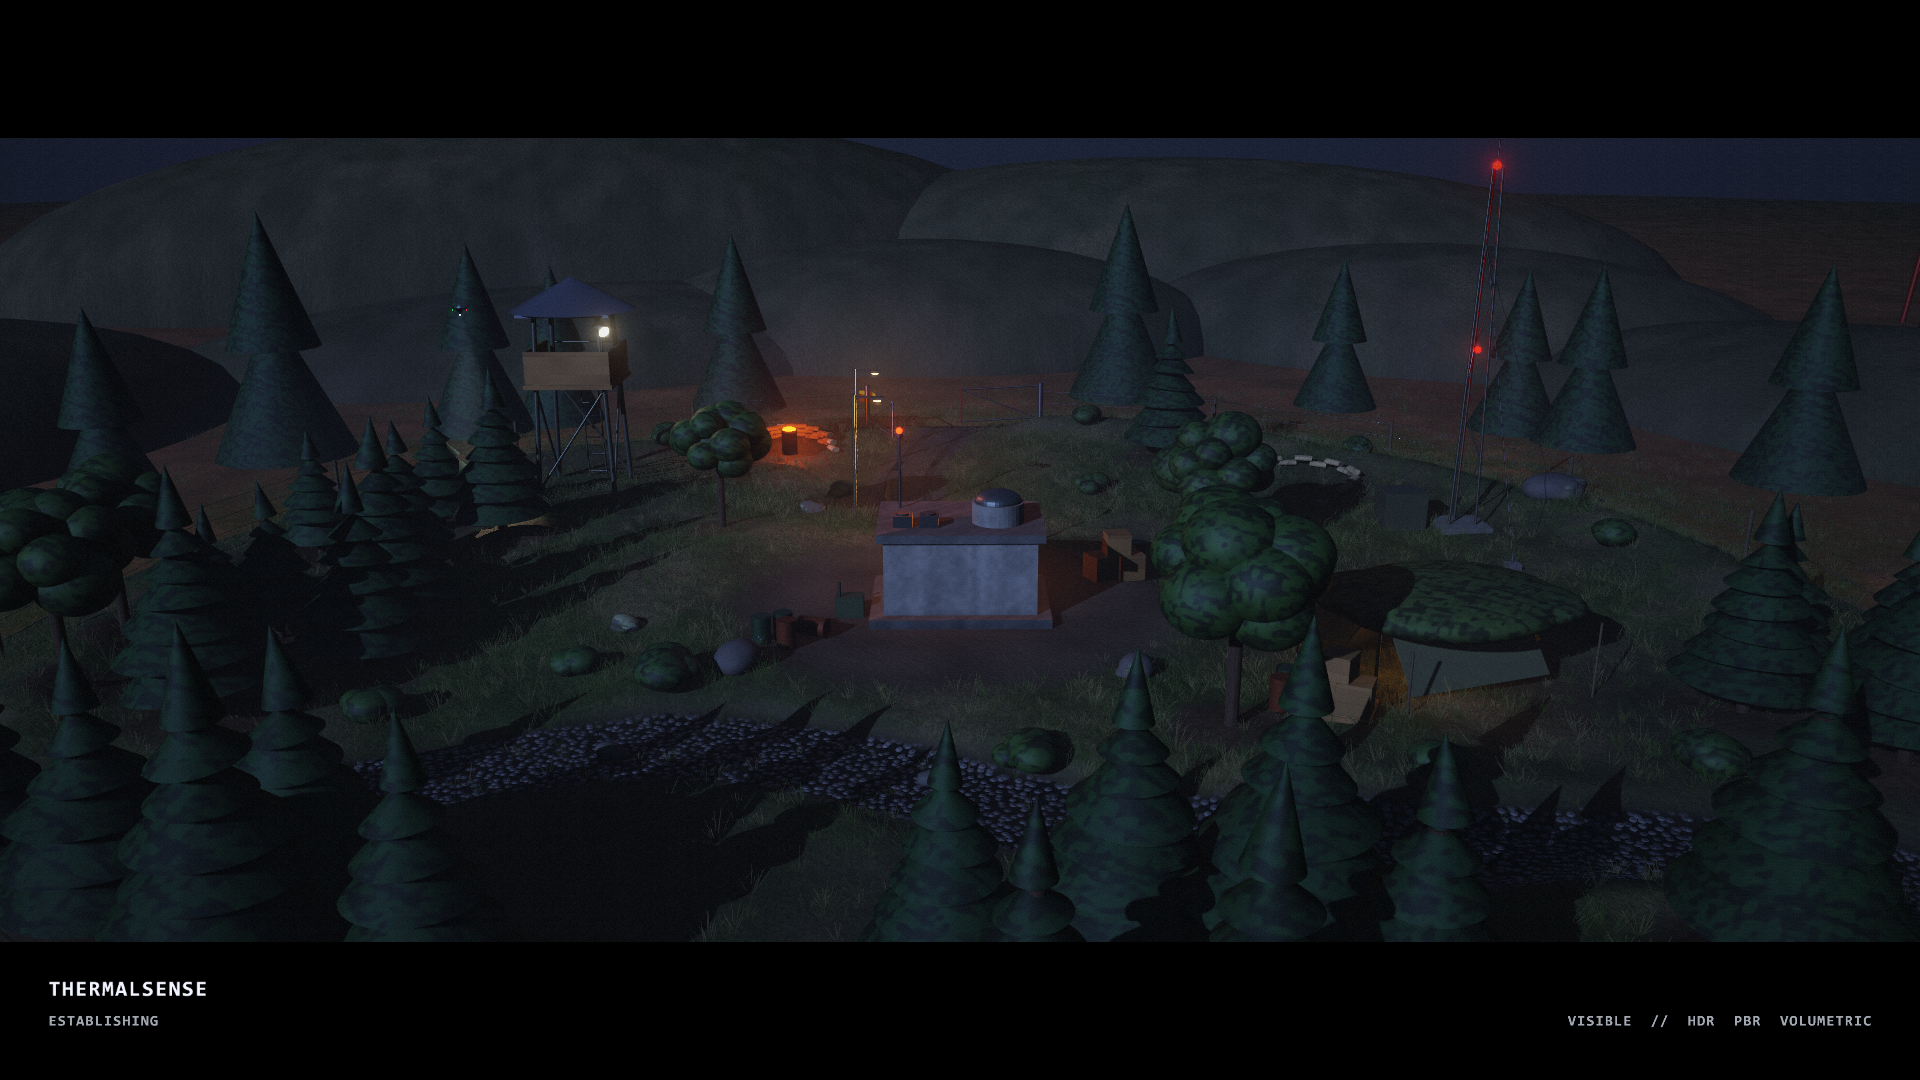
\includegraphics[width=\linewidth]{cine_establishing.png}
  \caption{The compound at night, rendered by the program (cinematic camera, \texttt{-{}-capture}). Every
  object in the image, from the pine forest to the fence wires and the grass, is made of the lab's
  unit primitives.}
  \label{fig:hero}
\end{figure}

% =====================================================================
\section{Introduction}
ThermalSense is an interactive OpenGL~3.3 simulation of a night patrol. A quadcopter UAV searches a
20\,m radius compound around a command bunker, finds a small ground robot \emph{from its own thermal
camera images} and follows it with a searchlight. The robot, in turn, plans routes that keep an
obstacle between itself and the UAV.

The lab assignment asks for primitives centred at the origin (cube, sphere, cylinder) and for every
object to be built from them with a documented scale/rotation/translation table. ThermalSense
follows this strictly. Three generators produce indexed unit meshes; the cone and the light
frustum are the same cylinder routine with a different top radius. Each mesh is uploaded to the GPU
once and all 805 parts of the scene are instances of these meshes under different model matrices.
No model files or image textures are used: surface detail is procedural. The only non-rigid surface
is the terrain, a cylinder cap subdivided into rings and displaced by a height function.

The second goal was a modern, realistic image. The renderer therefore adds a physically based
lighting model, shadow maps, ambient occlusion, volumetric fog, instanced grass and an HDR
post-processing chain (Sec.~\ref{sec:advanced}); each is measured by switching it off.

% =====================================================================
\section{Primitive Geometry Generation}
Every primitive is generated as a list of unique vertices $(x,y,z,n_x,n_y,n_z)$, 24 bytes each,
plus a triangle index list. Triangles are wound counter-clockwise when seen from outside, so with
\texttt{glFrontFace(GL\_CCW)} and back-face culling only outward faces are rasterised. The angular
resolution is $N=36$ slices, $\Delta\phi = 2\pi/36 = 10^\circ$, as in the lab sheet.

\begin{figure}[h]
  \centering
  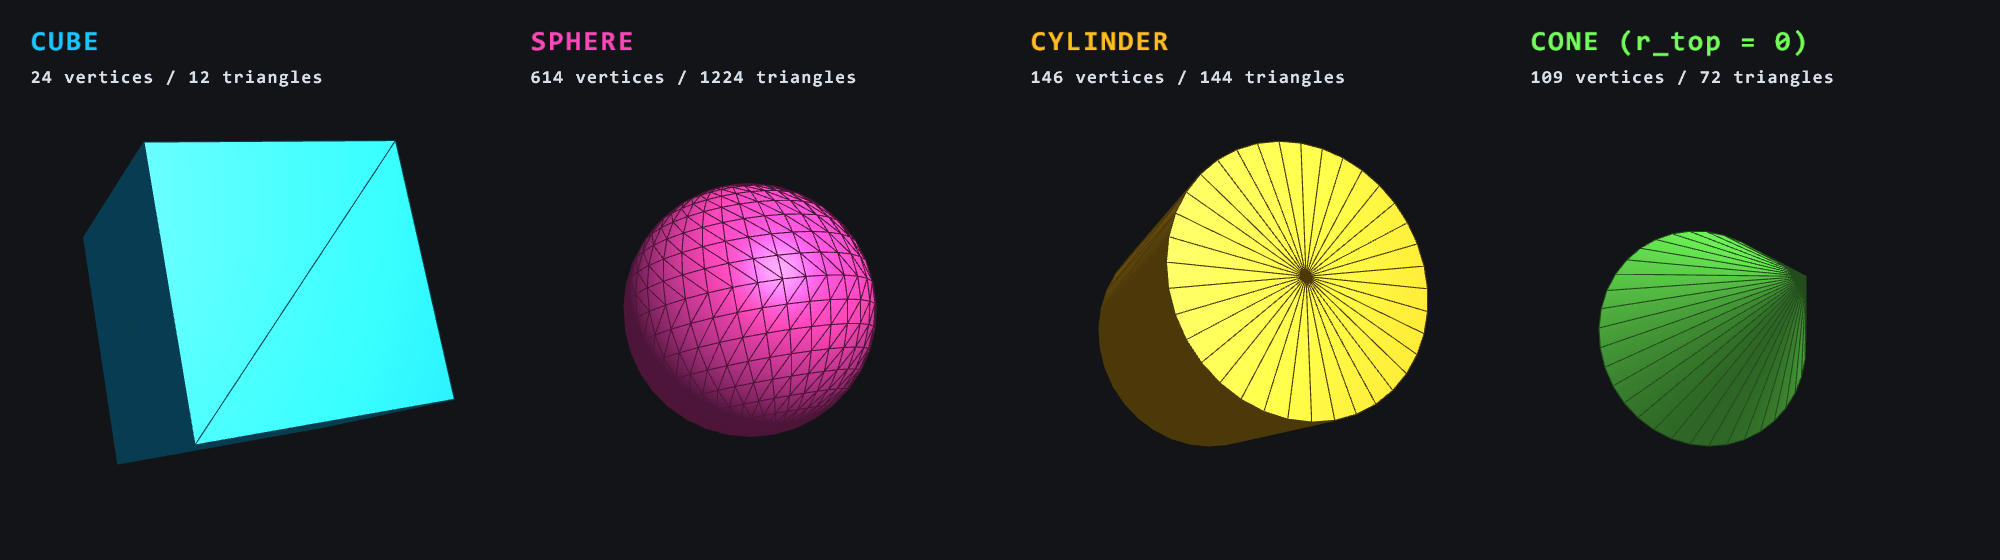
\includegraphics[width=\linewidth]{primitive_library.png}
  \caption{The primitive library rendered by the program with triangle edges on top. The counts are
  computed from the generators at capture time.}
  \label{fig:library}
\end{figure}

\subsection{Cube}
Each face has an outward normal $\vect n$ and in-plane axes $\vect u,\vect v$ with
$\vect u\times\vect v=\vect n$; its corners are
$\vect p_{c} = \tfrac12\vect n + \tfrac12 s_u\vect u + \tfrac12 s_v\vect v$ with
$(s_u,s_v)\in\{(-,-),(+,-),(+,+),(-,+)\}$, i.e.\ counter-clockwise about $\vect n$, and the face is
split into $(0,1,2)$ and $(0,2,3)$. A corner is stored once per face because its normal differs on
each face: 24 vertices, 36 indices, 12 triangles.

\subsection{Sphere}
With $r=0.5$, $\theta_k = k\pi/S$ and $\phi_j = 2\pi j/N$ ($S=18$, $N=36$):
$x = r\sin\theta_k\cos\phi_j,\ y = r\cos\theta_k,\ z = r\sin\theta_k\sin\phi_j,\ \vect n = \vect p/r$.
Only the northern hemisphere is computed (a fan around the pole plus quads between rings). The
southern half is its reflection $y\mapsto -y$, as sketched in the lab sheet. A reflection reverses
orientation, so each mirrored triangle $(a,b,c)$ is emitted as $(a',c',b')$. The equator is shared:
$2+(S-1)N = 614$ vertices and $2N(S-1)=1224$ triangles, with half the trigonometry.

\subsection{Cylinder, cone and frustum}
The axis is the local $z$ axis, $z\in[-0.5,0.5]$. The side joins two rings,
\begin{equation}
  \vect p^{\,b}_j=(r_b\cos\phi_j,\,r_b\sin\phi_j,\,-0.5),\quad
  \vect p^{\,t}_j=(r_t\cos\phi_j,\,r_t\sin\phi_j,\,+0.5),\quad
  \vect n_j=\mathrm{normalize}(\cos\phi_j,\,\sin\phi_j,\,r_b-r_t),
\end{equation}
and each cap is a fan around its own centre (normal $\pm\hat z$). With $r_b=r_t=0.5$ this is the lab cylinder: $4N+2=146$ vertices, $4N=144$
triangles. With $r_t=0$ the same routine gives the \textbf{cone} used for the pine whorls and roofs;
the collapsed top ring and top cap are skipped, leaving 109 vertices and 72 triangles with no
degenerate triangles. With $0<r_t<r_b$ and no caps it gives the searchlight frustum.

\noindent\textbf{Tests.} Unit tests check the counts, that every vertex lies in $[-0.5,0.5]^3$ and
is centred, that normals have unit length, and that no triangle is wound the wrong way (the geometric
normal $(\vect b-\vect a)\times(\vect c-\vect a)$ must agree with the stored normals). All 49
automated tests pass.

% =====================================================================
\section{Indexed Rendering and Optimisation}
Without indexing every triangle stores its three vertices (lab ``technique~1'': 18 floats for a
square); with indexing unique vertices go to the VBO and triangles reference them through the EBO
(technique~2: 12 floats $+\,6$ indices). The VAO records \emph{location~0: offset~0, stride~24\,B}
(position) and \emph{location~1: offset~12\,B} (normal). Memory per mesh is
$M_{\text{flat}} = 3T\cdot 24\,\text{B}$ and $M_{\text{indexed}} = 24V + 12T\,\text{B}$
(Table~\ref{tab:memory}). The six meshes take 923\,136\,B in total and are shared by all 805 parts;
in the main view indexed drawing submits 234\,310 vertices per frame instead of 1\,195\,980.

\begin{table}[h]
\centering\small
\caption{GPU meshes (exported by the program; the Excel workbook recomputes the byte columns with formulas).}
\label{tab:memory}
\begin{tabular}{lrrrrrrr}
\toprule
Mesh & $V$ & Indices & Triangles & Non-indexed (B) & Indexed (B) & Saving & Parts\\
\midrule
Cube & 24 & 36 & 12 & 864 & 720 & 16.7\,\% & 57\\
Sphere ($N{=}36,S{=}18$) & 614 & 3\,672 & 1\,224 & 88\,128 & 29\,424 & 66.6\,\% & 261\\
Cylinder ($N{=}36$) & 146 & 432 & 144 & 10\,368 & 5\,232 & 49.5\,\% & 261\\
Cone ($r_t=0$) & 109 & 216 & 72 & 5\,184 & 3\,480 & 32.9\,\% & 224\\
Light frustum & 72 & 216 & 72 & 5\,184 & 2\,592 & 50.0\,\% & 1\\
Terrain disc ($72\times256$) & 18\,433 & 109\,824 & 36\,608 & 2\,635\,776 & 881\,688 & 66.5\,\% & 1\\
\bottomrule
\end{tabular}
\end{table}

\textbf{Instancing and culling.} The grass is the unit cube drawn with
\texttt{glDrawElementsInstanced}: one VAO holds the cube's VBO/EBO plus a per-instance buffer
(root position, yaw, height, width, lean, seed) with \texttt{glVertexAttribDivisor}. 35\,000 blades
(High) cost one draw call per visible $10\times10$ grid cell instead of 35\,000 calls. Every pass
(main view, UAV camera, shadow maps, pre-pass) also culls parts whose bounding sphere
$r=\tfrac12\sqrt{s_x^2+s_y^2+s_z^2}$ lies outside one of the six frustum planes extracted from the
view-projection matrix (Gribb--Hartmann).

% =====================================================================
\section{Object Construction}\label{sec:construction}
A composite object is a small scene graph: leaves draw one primitive with their own $S,R,T$, group
nodes only carry a transform. The Excel sheet \emph{Object Construction} lists every node (934 rows,
805 leaves) and is generated from the same data as the program.
\begin{itemize}
  \item \textbf{Command bunker} (29 parts, flat): cube slab, block, roof, vestibule, door, glowing
  slits, vents and generator; cylinder turret ring, sandbags, mast and fan caps; sphere dome,
  beacon bulb (the point light) and door lamp.
  \item \textbf{UAV} (39 parts, Phong): cube fuselage, arms and blades; sphere canopy, hubs, LEDs and
  strobe; cylinder motors, struts, skids and four translucent rotor-blur discs. The searchlight is a
  hierarchy UAV $\rightarrow$ gimbal yaw $\rightarrow$ gimbal pitch $\rightarrow$ \{lamp, lens,
  camera, light frustum\}.
  \item \textbf{Rover} (26 parts, Phong): cube chassis, hull and motor box; six cylinder wheels
  (axis turned onto $x$ by $R_y(90^\circ)$, spin $=R_z$); sphere hubs, scanner and five IR sensors.
  \item \textbf{Environment} (621 parts, Gouraud): perimeter fence with wires and gate, watchtower
  with floodlight, sandbag walls, camouflage tent, supply caches, radio mast, lamp posts, fire barrel,
  boulders (3--4 rotated, squashed, half-buried spheres), bushes and forest. A spruce is a cylinder
  trunk with 5--7 drooping cone whorls, each slightly turned and tilted; a broadleaf tree is a trunk,
  three cylinder limbs (placed with a segment-aligned $R$) and 12 sphere clumps on a golden-angle
  spiral.
  \item \textbf{Terrain} (Gouraud): the cylinder cap subdivided into $K=72$ rings of $N=256$ points
  ($r_k=20k/K$), lifted to $y=h(x,z)$: rolling hills, a levelled pad under the bunker, a worn vehicle
  track, a dry creek bed and a berm inside the fence. \textbf{Backdrop} (89 parts): far ground,
  distant hills, a tree line and a far radio tower beyond the playable disc.
\end{itemize}

\begin{figure}[h]
  \centering
  \begin{subfigure}{0.245\linewidth}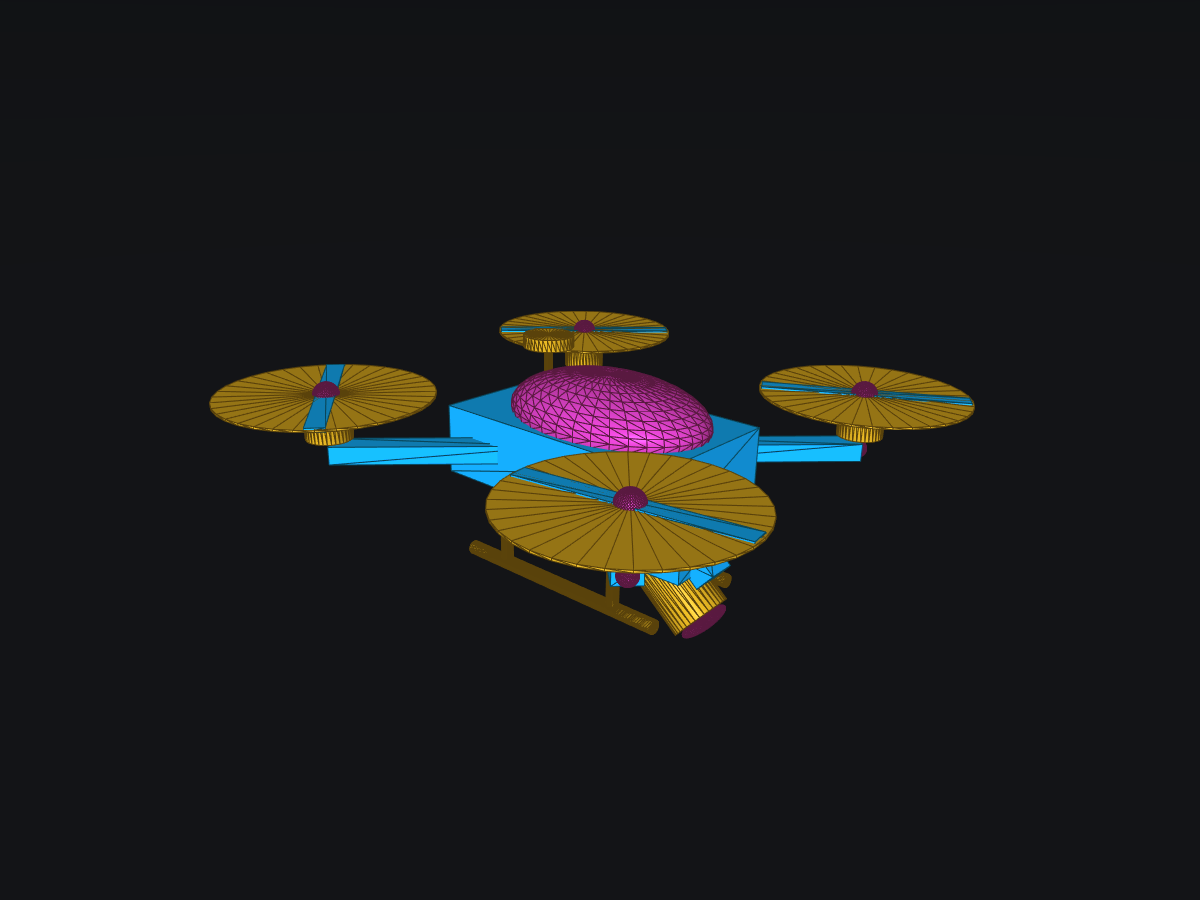
\includegraphics[width=\linewidth]{iso_uav_assembled.png}\caption{UAV}\end{subfigure}
  \begin{subfigure}{0.245\linewidth}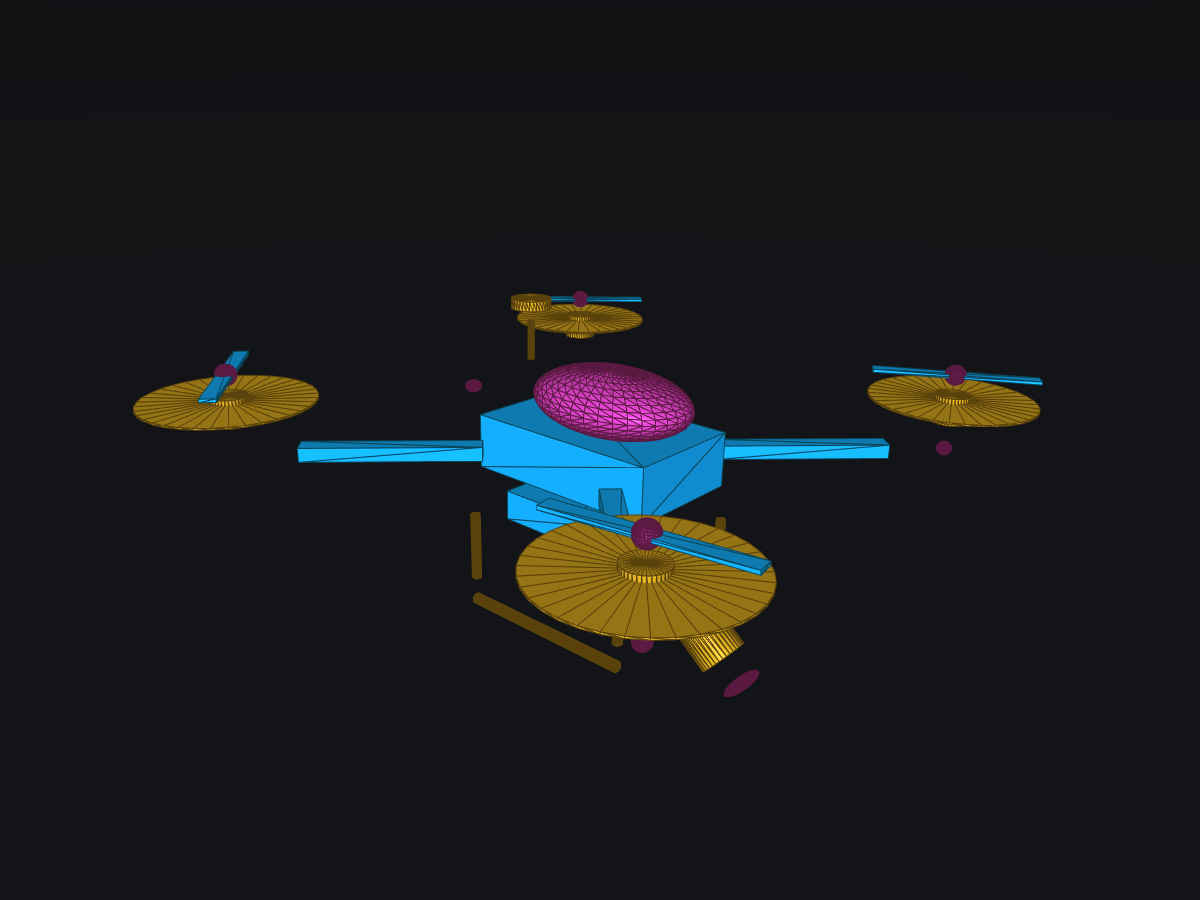
\includegraphics[width=\linewidth]{iso_uav_exploded.png}\caption{UAV, exploded}\end{subfigure}
  \begin{subfigure}{0.245\linewidth}
\includegraphics[width=\linewidth]{iso_rover_exploded.png}\caption{Rover, exploded}\end{subfigure}
  \begin{subfigure}{0.245\linewidth}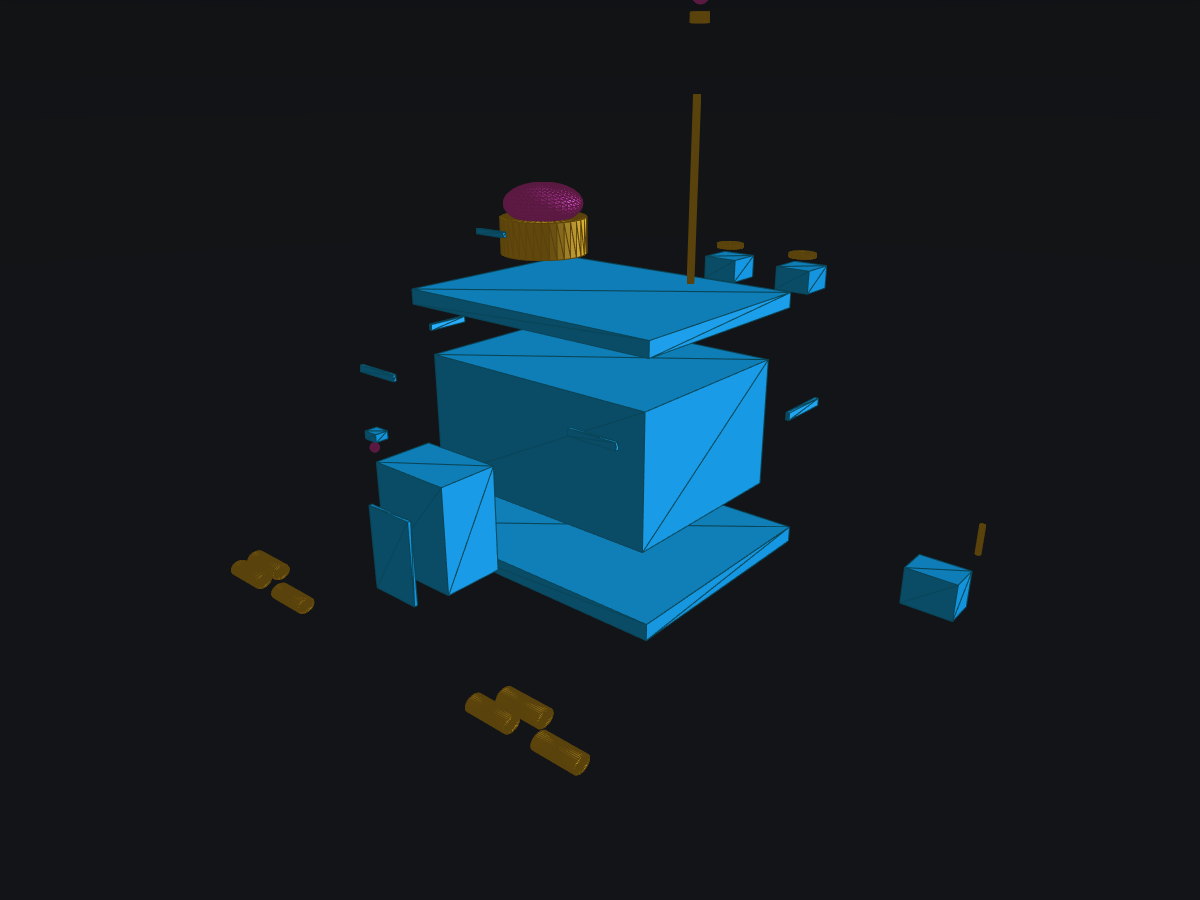
\includegraphics[width=\linewidth]{iso_bunker_exploded.png}\caption{Bunker, exploded}\end{subfigure}
  \caption{Construction view (keys \texttt{V}, \texttt{E}): cyan = cube, magenta = sphere, amber =
  cylinder, green = cone. In the explode view each part's translation is scaled by 1.7.}
  \label{fig:construction}
\end{figure}

% =====================================================================
\section{Transformations}
The model matrix of a node and its world matrix are
\begin{equation}
  M = T(\vect t)\,R_y(\psi)\,R_x(\theta)\,R_z(\varphi)\,S(\vect s),\qquad
  W_\text{node} = W_\text{parent}\,M ,
\end{equation}
\begin{equation}
  T=\begin{bmatrix}1&0&0&t_x\\0&1&0&t_y\\0&0&1&t_z\\0&0&0&1\end{bmatrix},\;
  S=\begin{bmatrix}s_x&0&0&0\\0&s_y&0&0\\0&0&s_z&0\\0&0&0&1\end{bmatrix},\;
  R_y(\psi)=\begin{bmatrix}\cos\psi&0&\sin\psi&0\\0&1&0&0\\-\sin\psi&0&\cos\psi&0\\0&0&0&1\end{bmatrix}.
\end{equation}
The primitive is scaled first, then rotated about its own centre, then placed; the other order would
scale the translation too (test T14: $(1,0,0)\xrightarrow{S(2)}(2,0,0)\xrightarrow{R_z(90^\circ)}
(0,2,0)\xrightarrow{T(1,2,3)}(1,4,3)$). Normals use $(M^{-1})^{T}$. The Excel sheet
\emph{Transformation Matrices} rebuilds $T$, $R$, $S$ and $M=TRS$ for all 805 parts with cell
formulas (the ``M1, M2, M3'' table of the lab sheet) and compares them with the matrices exported by
the code: the largest difference is $1.7\times10^{-5}$. The searchlight shows the hierarchy:
$W_\text{lamp} = W_\text{UAV}\,M_\text{yaw}(\psi_g)\,M_\text{pitch}(\theta_g)$; the spotlight sits
at the lens of $W_\text{lamp}$ and points along its local $+z$ axis.

\begin{figure}[h]
\centering
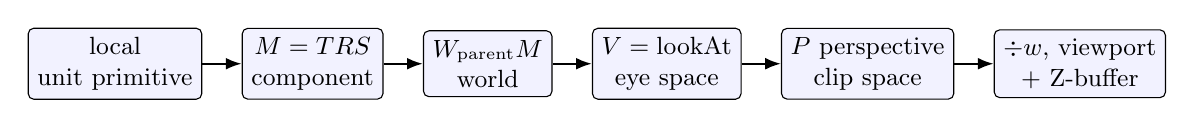
\begin{tikzpicture}[node distance=4mm and 5mm, every node/.style={font=\small},
  box/.style={draw,rounded corners=2pt,minimum height=6.5mm,align=center,fill=blue!5},
  arr/.style={-{Latex[length=2mm]},thick}]
  \node[box] (a) {local\\unit primitive};
  \node[box,right=of a] (b) {$M=TRS$\\component};
  \node[box,right=of b] (c) {$W_\text{parent}M$\\world};
  \node[box,right=of c] (d) {$V=\text{lookAt}$\\eye space};
  \node[box,right=of d] (e) {$P$ perspective\\clip space};
  \node[box,right=of e] (f) {$\div w$, viewport\\+ Z-buffer};
  \foreach \x/\y in {a/b,b/c,c/d,d/e,e/f} \draw[arr] (\x)--(\y);
\end{tikzpicture}
\caption{Vertex pipeline: $\vect p_\text{clip} = P\,V\,W_\text{parent}\,T R S\,\vect p_\text{local}$.}
\label{fig:transform}
\end{figure}

% =====================================================================
\section{Shading and Lighting}\label{sec:shading}
\textbf{Where lighting is evaluated.} Flat, Gouraud and Phong differ in \emph{where} the lighting
model is evaluated. \emph{Flat} (bunker): a geometry shader computes one normal per triangle,
$\vect N_f=\mathrm{normalize}((\vect p_1-\vect p_0)\times(\vect p_2-\vect p_0))$, and lights the
triangle once at its centroid. \emph{Gouraud} (terrain, vegetation, props): lighting in the vertex
shader, interpolated. \emph{Phong} (UAV, rover): the normal is interpolated and lighting is
evaluated per fragment. Each light's diffuse and specular terms are kept separate across the stages,
so shadows and ambient occlusion (visibility, not lighting) can still be applied per fragment.

\textbf{Lighting model.} The visible view uses the Cook--Torrance microfacet BRDF with roughness
$\alpha=\rho^2$ and metalness $m$ per material:
\begin{equation}
  f_s = \frac{D\,G\,F}{4(\vect N\!\cdot\!\vect V)(\vect N\!\cdot\!\vect L)},\quad
  D=\frac{\alpha^2}{\pi\big((\vect N\!\cdot\!\vect H)^2(\alpha^2-1)+1\big)^2},\quad
  F=F_0+(1-F_0)(1-\vect V\!\cdot\!\vect H)^5,
\end{equation}
with Smith--Schlick $G$, $F_0=\mathrm{mix}(0.04,\text{albedo},m)$ and diffuse $(1-F)(1-m)$. Key
\texttt{B} switches back to the classic Blinn--Phong
$k_d(\vect N\!\cdot\!\vect L)+k_s(\vect N\!\cdot\!\vect H)^n$ of the proposal. Ambient light is a
sky/ground hemisphere.

\textbf{Lights.} L0 directional moonlight; L1 the bunker beacon, a point light with
$f=1/(1+0.35d+0.45d^2)$ pulsing at 1\,Hz; L2 the UAV spotlight with
$f=c^2/(1+0.05d+0.03d^2)$, $c=\mathrm{clamp}\big((\cos\gamma-\cos14^\circ)/(\cos9^\circ-\cos14^\circ)\big)$.
Keys \texttt{1}--\texttt{3} toggle them. In addition, up to eight \emph{practical lights} (door
lamp, sodium lamp posts, fire barrel, tent lantern, watchtower floodlight, aviation lights, UAV
strobe) are emissive parts whose material is also a light, with the windowed falloff
$f=\mathrm{saturate}(1-(d/R)^4)^2/(1+d^2)$. They give the warm/cool contrast of
Fig.~\ref{fig:results}.

\textbf{Procedural surfaces and the ground.} Albedo detail comes from value noise and cellular noise
in the shader (concrete streaks, painted chips, bark, rock lichen, leaf clusters). The ground uses a
$512\times512$ data map computed once on the CPU from the scene layout (creek wetness, track, forest
floor under the crowns, meadow density); the grass placement uses the same map. The terrain shader
mixes turf, compacted track with two tyre ruts, a wet pebble creek bed (cellular noise) and needle
litter. A small height field $h(x,z)$ (clods, pebbles, ruts) gives a detail normal $\vect N_d$ by
central differences. Its effect on the per-vertex (Gouraud) irradiance $E_v$ is the ratio
$E=E_v\,\frac{\max(\vect N_d\cdot\vect L,0)+\epsilon}{\max(\vect N\cdot\vect L,0)+\epsilon}$, so the
lighting stays per vertex while the relief shows per pixel. Wet areas get their own glossy GGX
highlight and a sky reflection.

\textbf{Thermal view.} Each material has an intrinsic temperature $h_0$ (ground 0.15, bunker 0.34,
rover motor 0.97). The displayed heat is $h=h_0+0.04\min(E,1.5)$ plus low-frequency ground noise. The
light term is small and capped on purpose: a long-wave IR camera hardly sees visible light. Key
\texttt{T} switches the colour map between ironbow, white-hot and rainbow; the main view, the UAV
feed and the HUD scale use the same stops (Fig.~\ref{fig:weather}c).

\textbf{Thermal footprints.} The rover leaves heat on the ground: a $256\times256$ grid over the disc
(15.6\,cm cells) receives $\Delta T = 2.2\,|v_\text{wheel}|\,\Delta t$ under each wheel (tyre
friction, proportional to the distance rolled) and a small constant under the hull while parked
(engine heat). The grid cools exponentially, $T(t)=T_0e^{-t/\tau}$ with $\tau=45$\,s on dry ground
and 15\,s when soaked. It is uploaded every frame as a texture and adds up to 0.28 to the ground's
heat, so the hottest track (0.51) stays below the tracker's 0.80 blob threshold: the UAV camera sees
the tracks (Fig.~\ref{fig:weather}d) but they can never be mistaken for the rover (tests T47--T49;
the 180\,s behaviour trace is unchanged).

% =====================================================================
\section{Advanced Rendering}\label{sec:advanced}
The frame is rendered in linear light into a multisampled HDR target
(\texttt{GL\_R11F\_G11F\_B10F}, $4\times$ MSAA on High) and tone-mapped at the end:

\begin{figure}[h]
\centering
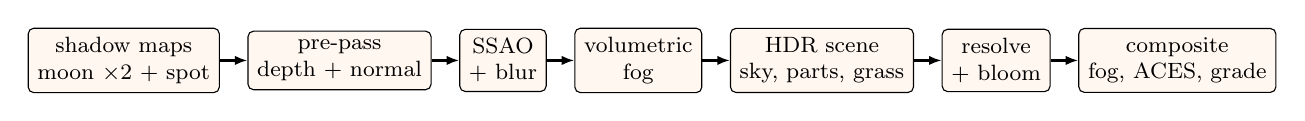
\begin{tikzpicture}[node distance=3mm and 3.5mm, every node/.style={font=\footnotesize},
  box/.style={draw,rounded corners=2pt,minimum height=6.5mm,align=center,fill=orange!6},
  arr/.style={-{Latex[length=1.6mm]},thick}]
  \node[box] (s) {shadow maps\\moon $\times2$ + spot};
  \node[box,right=of s] (p) {pre-pass\\depth + normal};
  \node[box,right=of p] (a) {SSAO\\+ blur};
  \node[box,right=of a] (f) {volumetric\\fog};
  \node[box,right=of f] (m) {HDR scene\\sky, parts, grass};
  \node[box,right=of m] (b) {resolve\\+ bloom};
  \node[box,right=of b] (c) {composite\\fog, ACES, grade};
  \foreach \x/\y in {s/p,p/a,a/f,f/m,m/b,b/c} \draw[arr] (\x)--(\y);
\end{tikzpicture}
\caption{The v2 frame. The UAV camera image for the computer vision is rendered separately, without post-processing.}
\label{fig:frame}
\end{figure}

\textbf{Shadow maps.} The moon uses two orthographic cascades in a depth-texture array: a near
cascade fitted around the bounding sphere of the view-frustum slice $[z_n, 12\,\text{m}]$ and a
world cascade around the whole disc ($r=23$\,m, 2.25\,cm per texel at $2048^2$). To stop shadow
edges shimmering, the cascade centre is snapped to whole texels in light space,
$c'=\lfloor c/\Delta\rfloor\Delta$ with $\Delta=2r/\text{res}$ (test T34: a camera move shifts the map
by whole texels only). The world cascade never moves, so its static casters are rendered once into a
cache that is copied in every frame before the UAV and rover are drawn on top. The searchlight has a
perspective shadow map along the lamp axis. Lookups use a normal-offset bias and a rotated Poisson
disc of 8 (High) or 16 (Ultra) hardware-PCF taps. \textbf{SSAO} samples a normal-oriented hemisphere
around each pixel of a half-resolution depth/normal pre-pass and is blurred depth-aware.
\textbf{Volumetric fog} ray-marches a height fog $\sigma(y)=\sigma_0e^{-0.22y}$ lit by the moon, the
beacon and the practical lights with single scattering,
$L \mathrel{+}= T\,L_\text{in}(1-e^{-\sigma\Delta s})$, $T\mathrel{*}=e^{-\sigma\Delta s}$. The
searchlight shaft is a thin cone that a coarse march would miss, so the ray is intersected
analytically with the cone $(\vect d\cdot\vect a)^2=\cos^2\gamma\,|\vect x-\vect s|^2$ (a quadratic
in $t$) and only that interval is sampled, with the spot shadow map (Fig.~\ref{fig:results}d).
\textbf{Bloom} uses a soft-knee threshold, a 13-tap downsample chain and a tent upsample.
\textbf{Composite:} fog, bloom, exposure, colour grading, the ACES filmic curve
$\frac{x(2.51x+0.03)}{x(2.43x+0.59)+0.14}$, gamma, vignette and grain.

\textbf{Rain} (key \texttt{R}). 14\,000 streaks (High) are the unit cube, instanced and stretched along
the fall direction by the distance a drop falls in $1/40$\,s. The drops live in a $24\times14\times24$\,m box
that wraps around the camera in the vertex shader, $\vect x=\vect o+\big((\vect p-\vect o)\bmod\vect b\big)$,
so the rain never runs out. They are blended additively and lit with forward scattering, which makes
them glow in front of the lamps and inside the searchlight cone. A wetness value builds up over
about 20\,s and dries over 90\,s. It darkens porous materials by up to 45\,\%, puts a water film
($\rho\rightarrow0.25\rho$) on up-facing surfaces, grows puddles in hollows and ruts with ripple
rings from random impacts, and adds per-fragment GGX reflections of the practical lights on wet
ground. The sky becomes overcast (clouds close, stars and moon fade), the moonlight drops by 55\,\%
and the fog density rises. In the thermal view the rain is invisible, as it is to a long-wave camera,
but wet surfaces read cooler and the tracks evaporate faster (Fig.~\ref{fig:weather}).

\begin{figure}[h]
  \centering
  \begin{subfigure}{0.495\linewidth}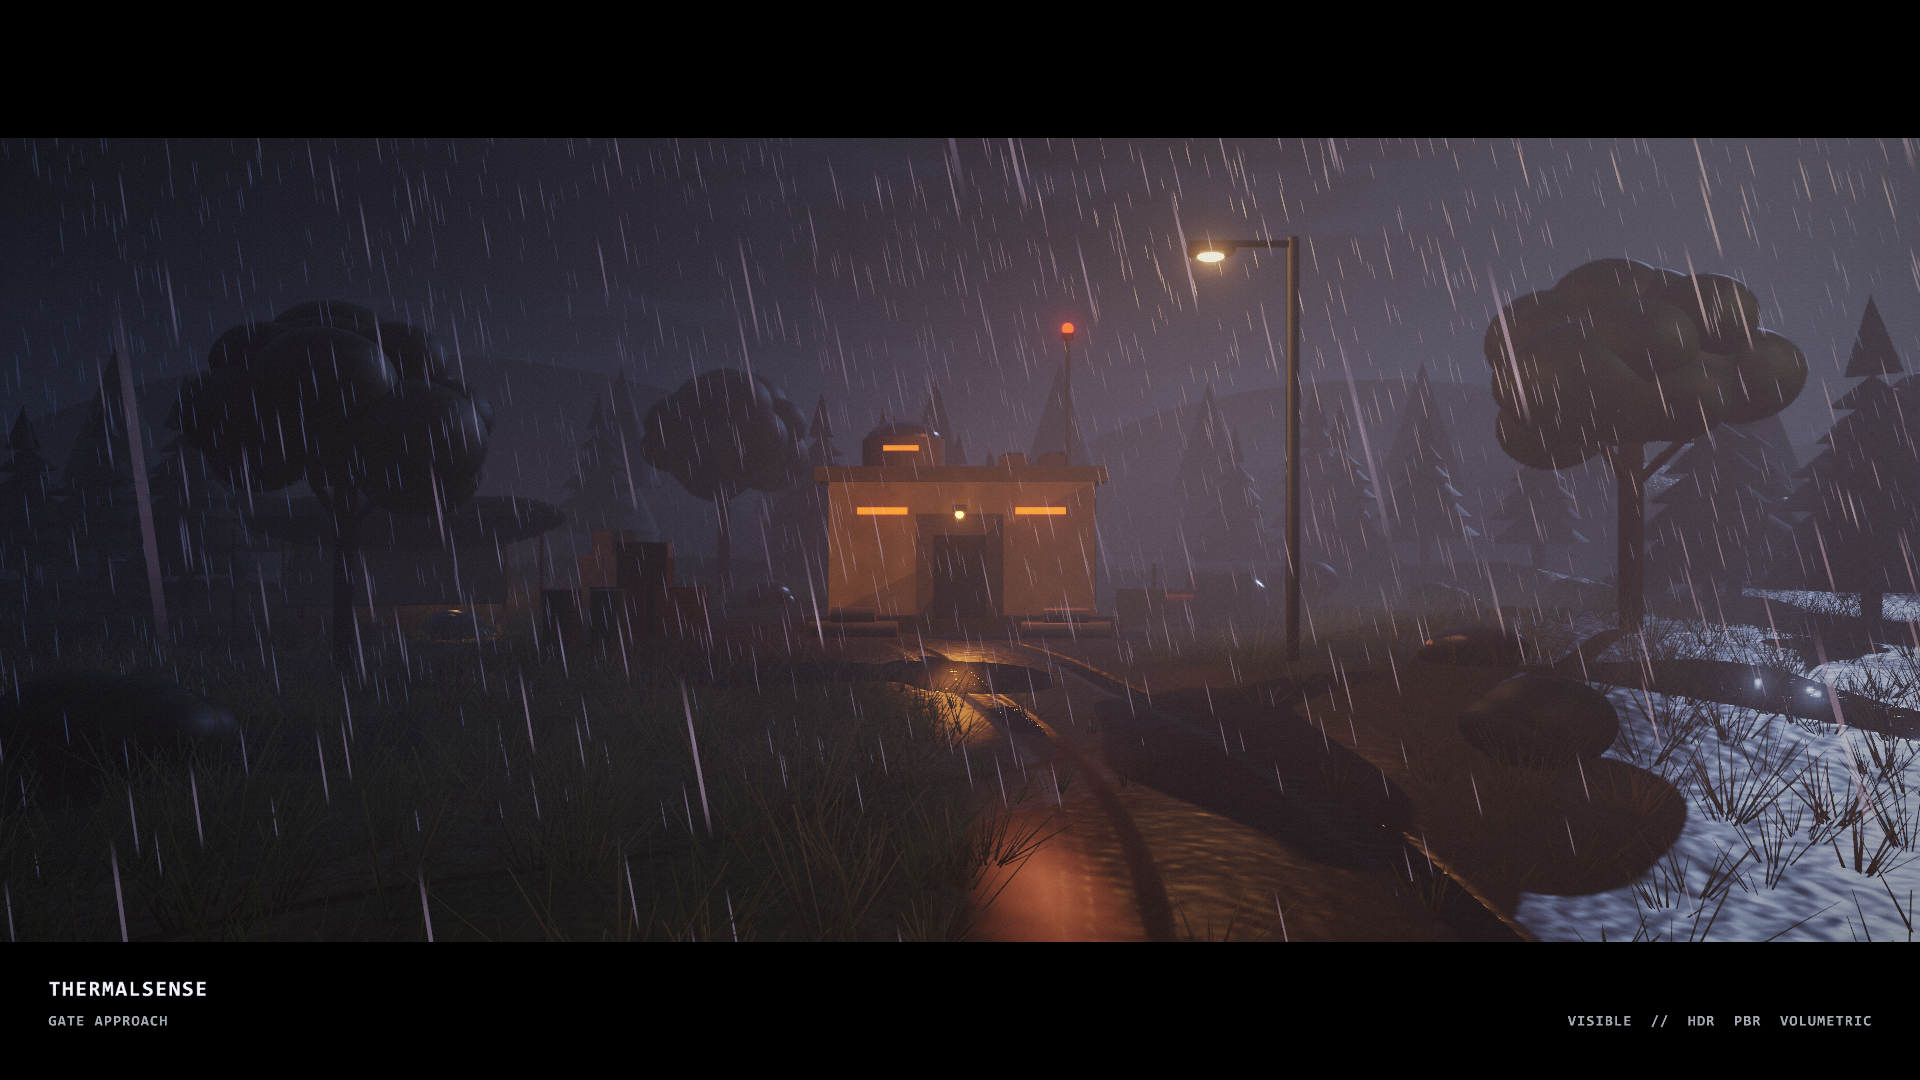
\includegraphics[width=\linewidth]{rain_gate.png}\caption{Rain: lamp light on the wet ruts}\end{subfigure}
  \begin{subfigure}{0.495\linewidth}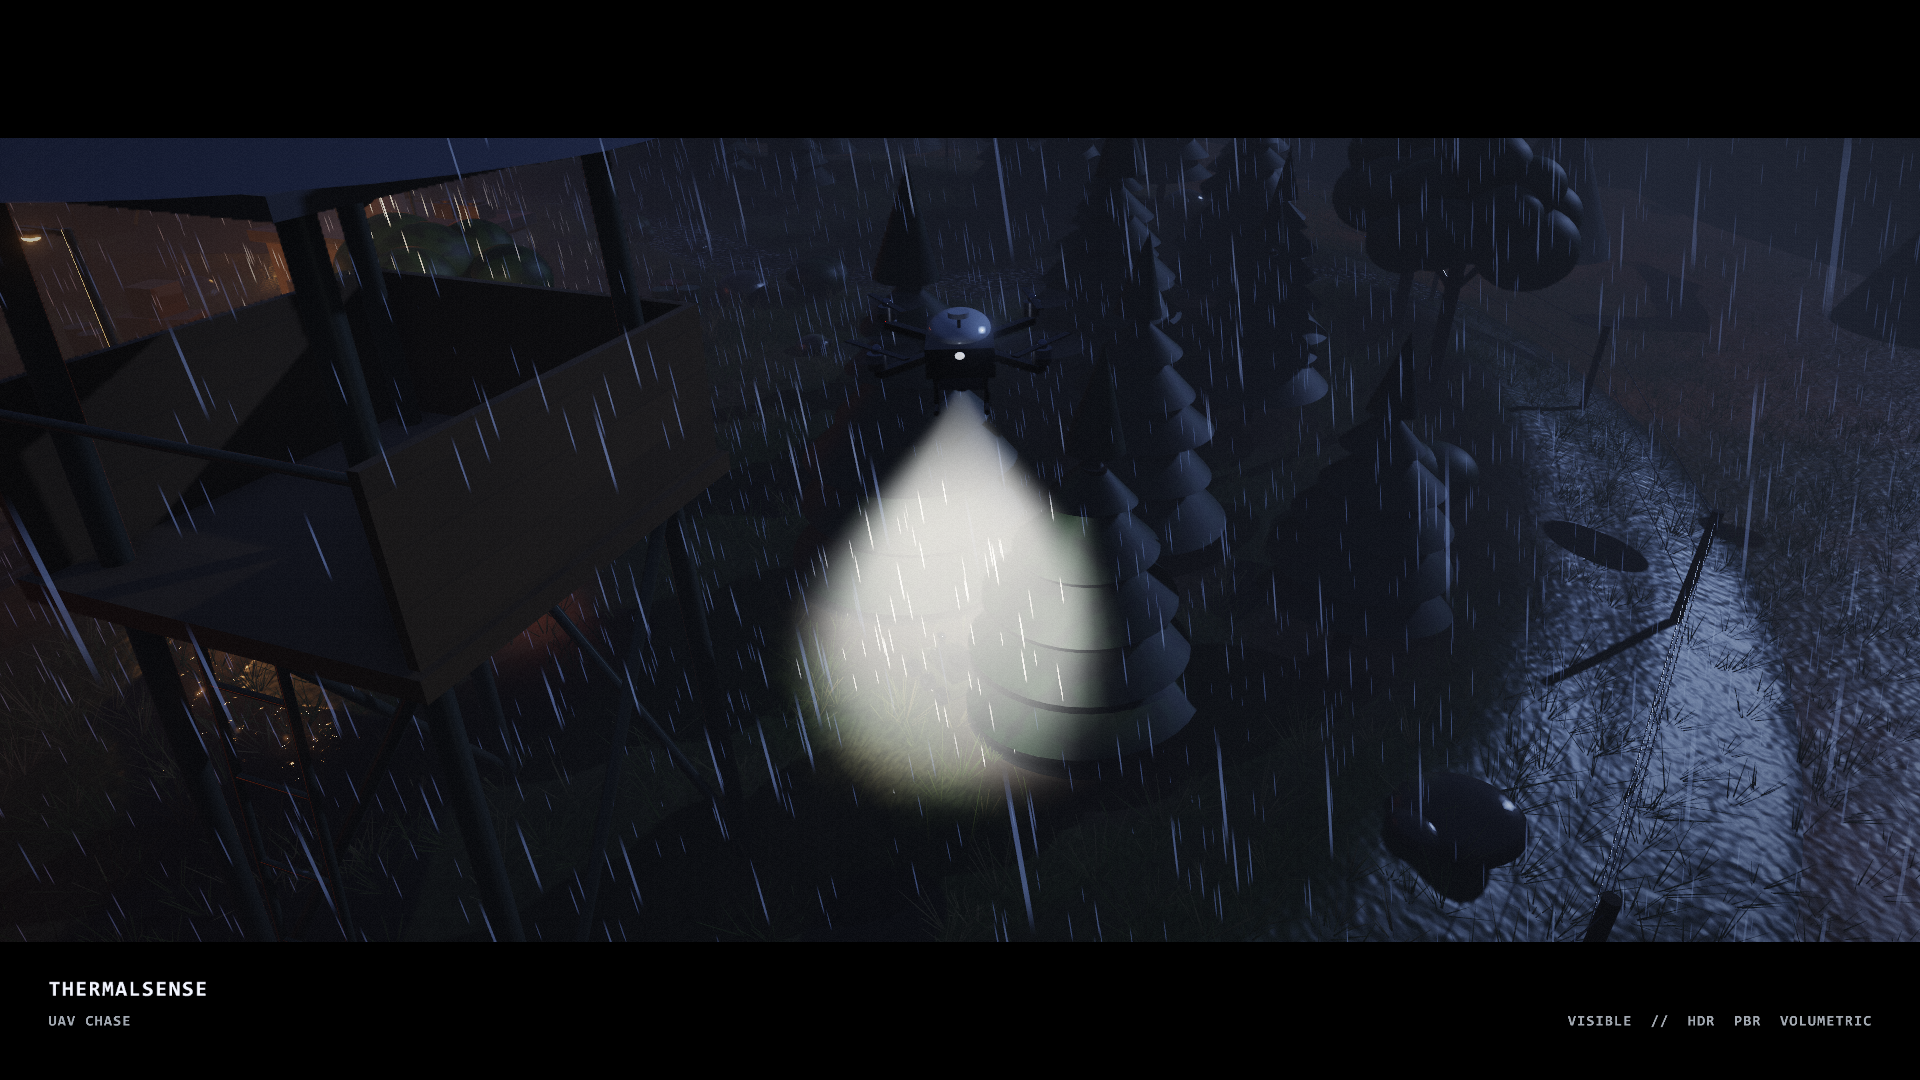
\includegraphics[width=\linewidth]{rain_chase.png}\caption{Rain in the searchlight}\end{subfigure}\\[1mm]
  \begin{subfigure}{0.325\linewidth}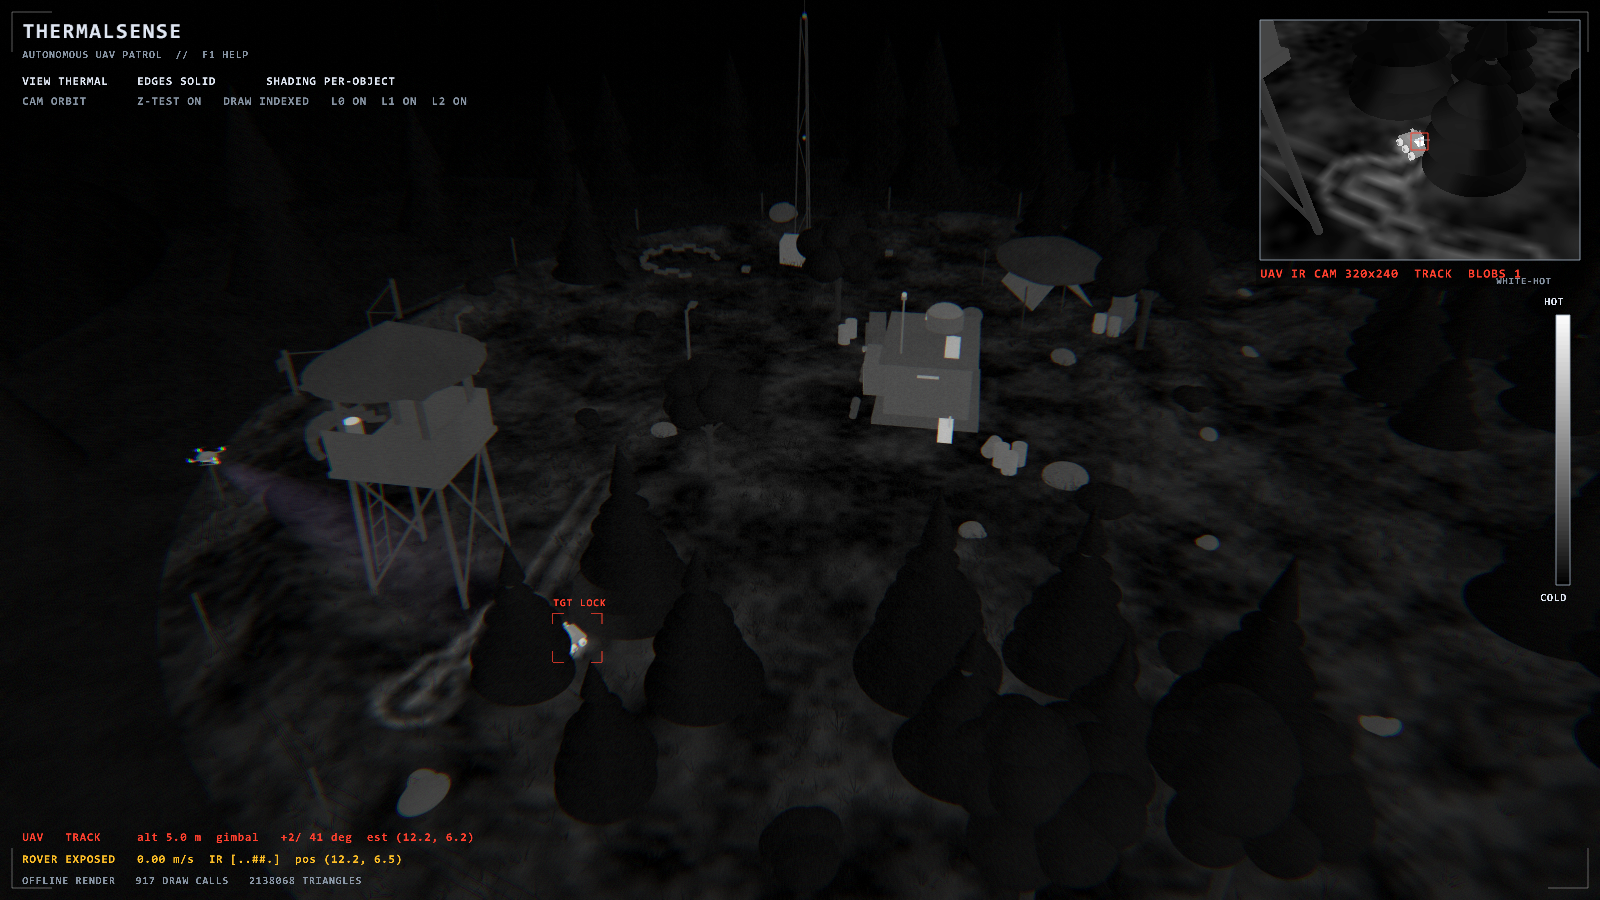
\includegraphics[width=\linewidth]{scene_thermal_whitehot.png}\caption{White-hot palette}\end{subfigure}
  \begin{subfigure}{0.325\linewidth}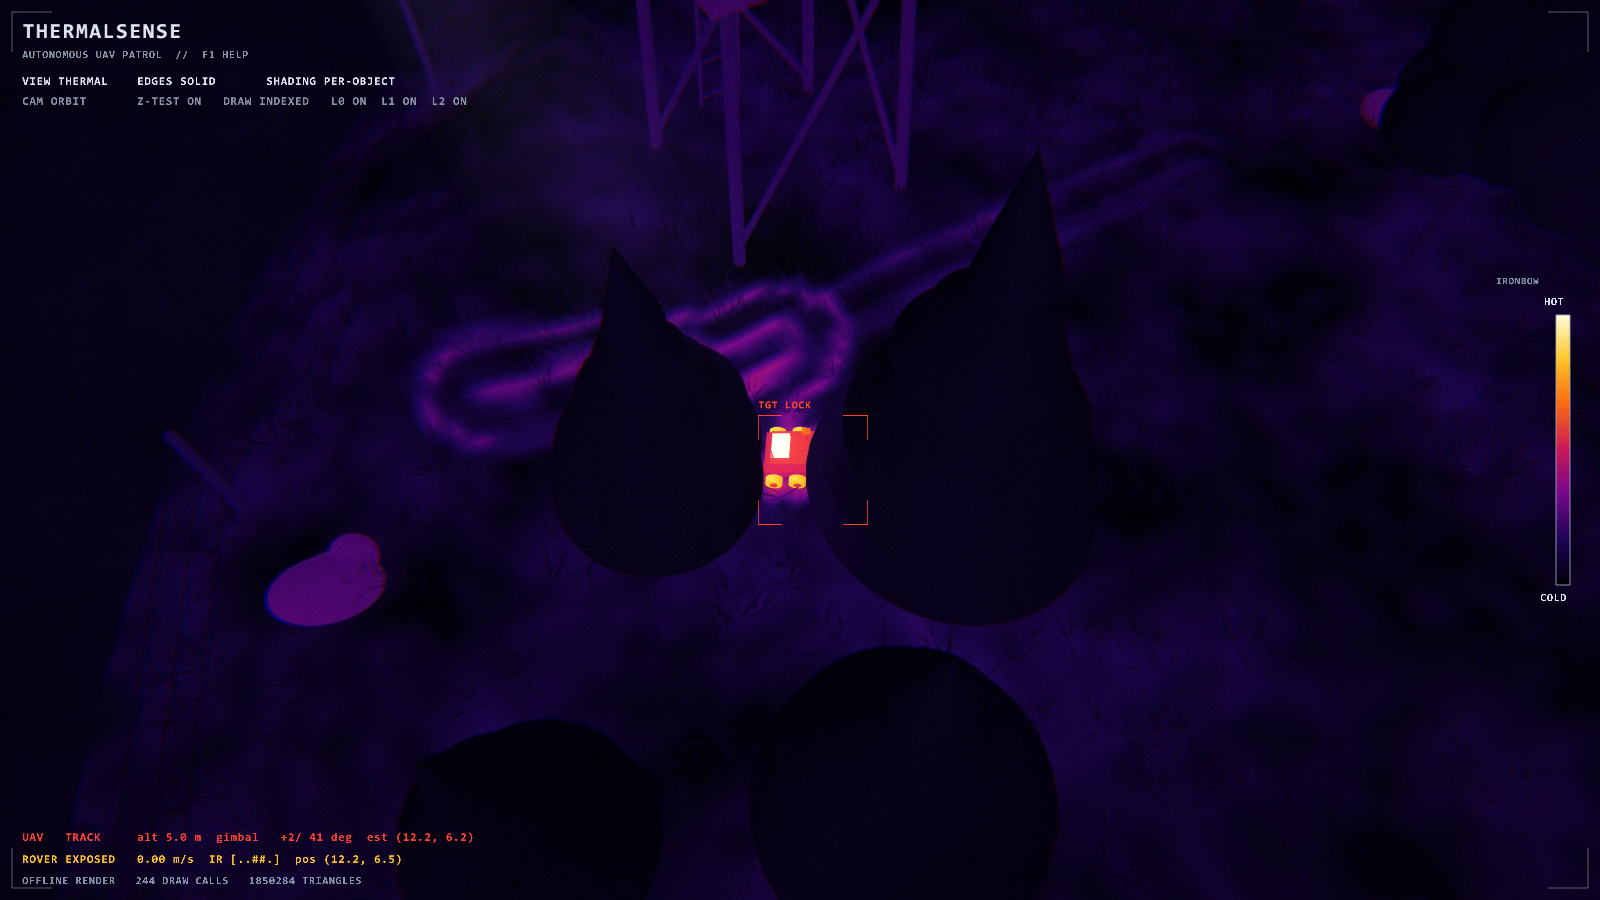
\includegraphics[width=\linewidth]{thermal_footprints.png}\caption{Rover's warm tyre tracks}\end{subfigure}
  \begin{subfigure}{0.325\linewidth}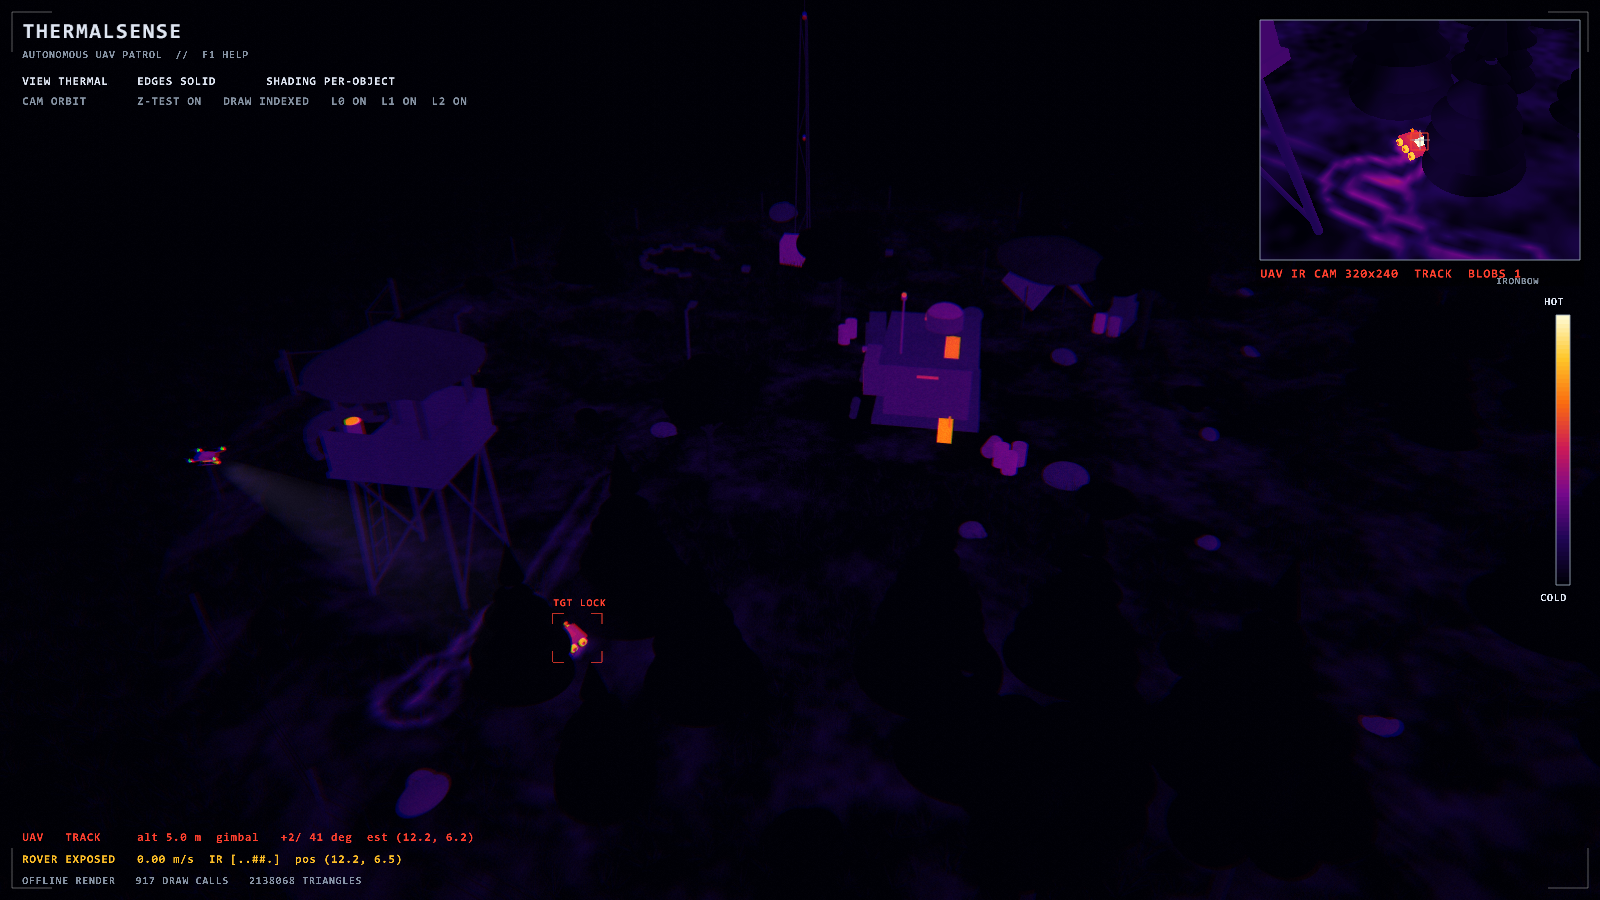
\includegraphics[width=\linewidth]{rain_thermal.png}\caption{Thermal view in rain}\end{subfigure}
  \caption{Weather and thermal features: rain in the visible view, a second thermal palette, thermal
  footprints, and the rain-cooled thermal view in which the tracks stand out.}
  \label{fig:weather}
\end{figure}

\begin{figure}[h]
  \centering
  \begin{subfigure}{0.325\linewidth}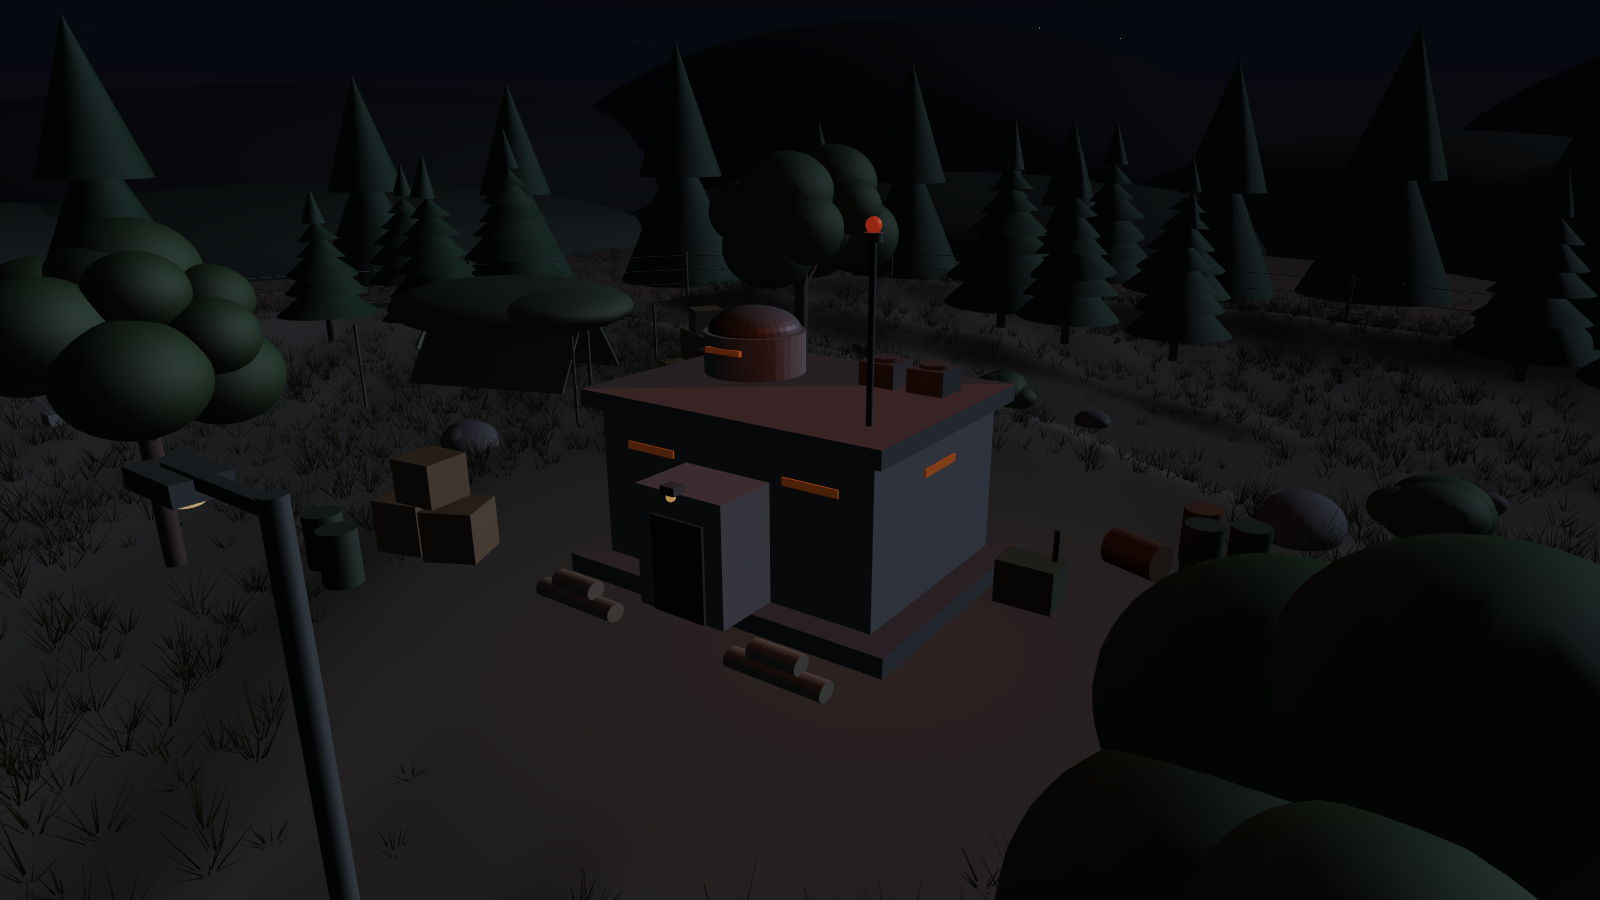
\includegraphics[width=\linewidth]{compare_v1.png}\caption{v1 renderer}\end{subfigure}
  \begin{subfigure}{0.325\linewidth}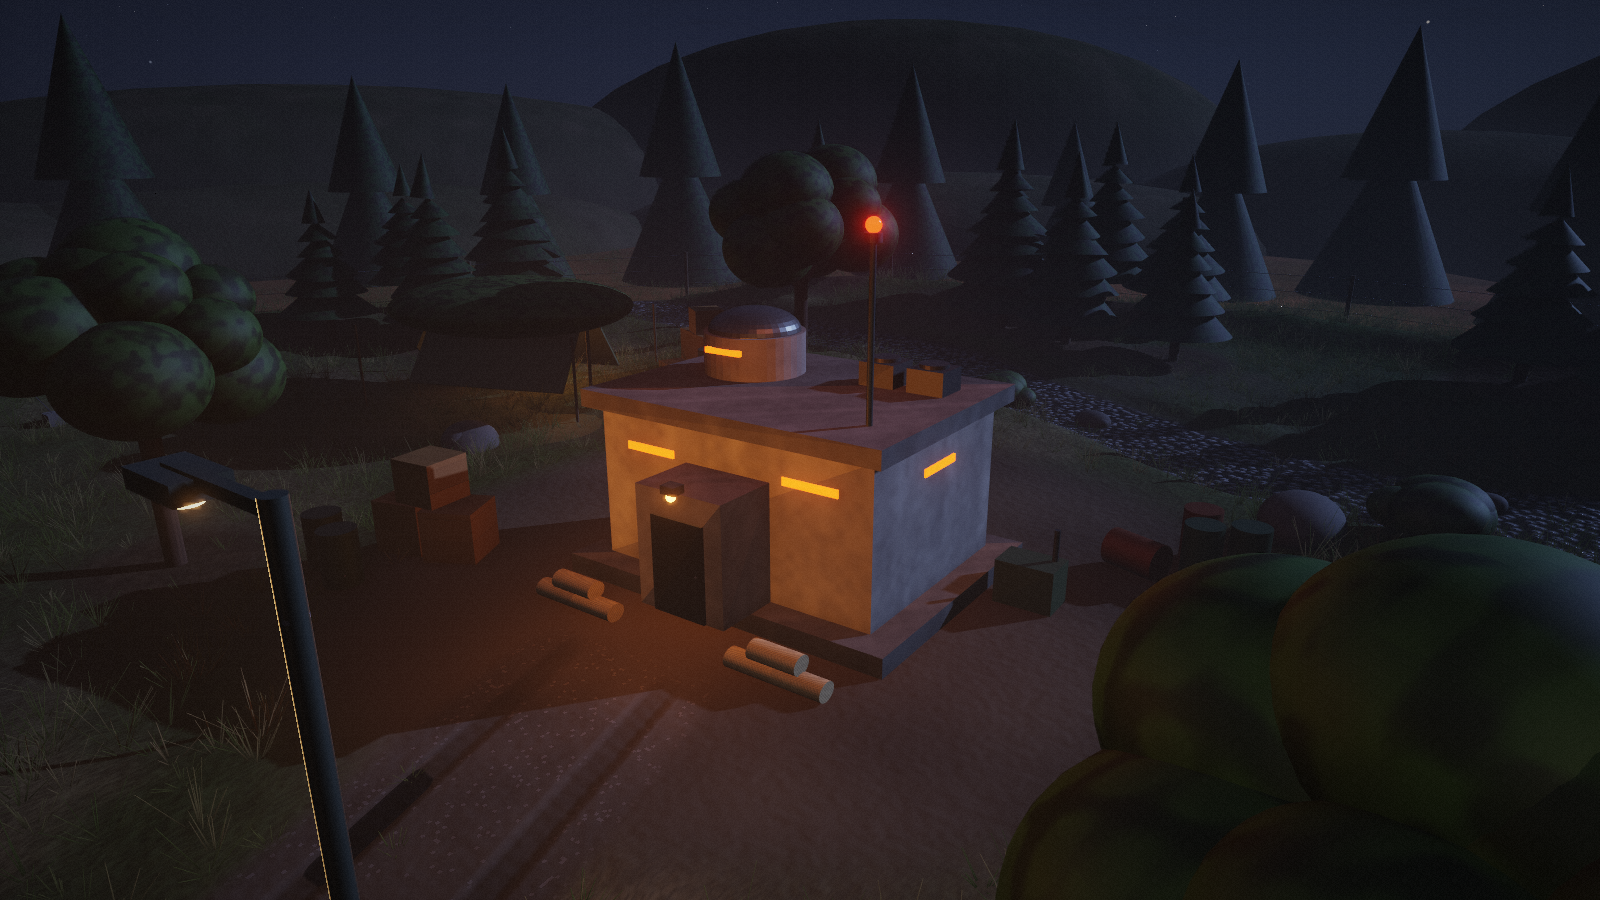
\includegraphics[width=\linewidth]{compare_v2.png}\caption{v2 pipeline}\end{subfigure}
  \begin{subfigure}{0.325\linewidth}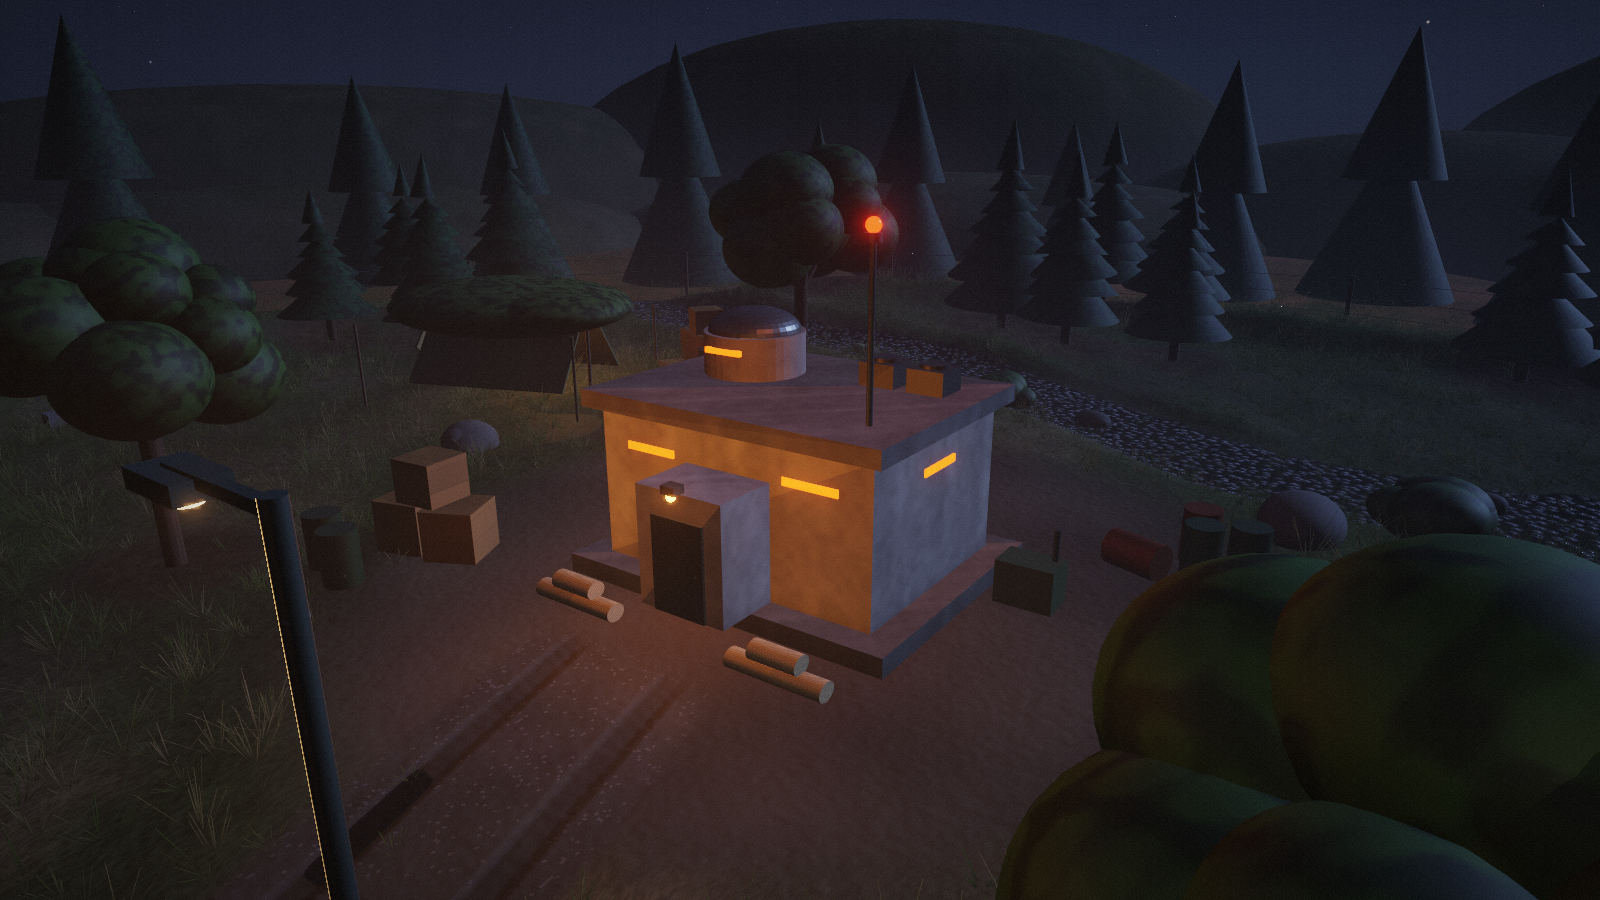
\includegraphics[width=\linewidth]{ablate_shadows.png}\caption{v2 without shadow maps}\end{subfigure}
  \caption{Same camera, same simulation time. (a) the v1 renderer (Blinn--Phong, no post-processing,
  key \texttt{N}); (b) the full pipeline; (c) the pipeline with shadow maps switched off.}
  \label{fig:compare}
\end{figure}

\begin{table}[h]
\centering\small
\caption{Measured frame cost ($1280\times720$, AMD Radeon integrated GPU, \texttt{-{}-benchmark}: median of 5
interleaved rounds at high process priority). Feature cost = difference to High; it counts as resolved when it is
larger than the interquartile range of the rounds (5.2\,ms for High).}
\label{tab:cost}
\begin{tabular}{lrr@{\qquad}lrl}
\toprule
Preset & FPS & ms/frame & Feature (High) & cost (ms) & \\
\midrule
v1 renderer & 32.2 & 31.0 & shadow maps & 16.2 & resolved\\
Low & 18.2 & 55.0 & MSAA $4\times$ & 9.3 & resolved\\
High & 14.7 & 67.9 & rain (added) & 7.1 & resolved\\
High, non-indexed & 14.3 & 70.1 & volumetric fog & 2.9 & below noise\\
Ultra (captures, video) & 4.9 & 202.7 & searchlight shadow & 2.6 & below noise\\
 & & & SSAO / bloom & 1.3 / 0.7 & below noise\\
\bottomrule
\end{tabular}
\end{table}

The integrated GPU of the test machine is the limit. The interactive presets trade features for
speed (key \texttt{F5}), while the report figures and the demo video (\texttt{-{}-record}) are
rendered offline on Ultra. Shadow maps are the most expensive feature, even with culling and the
static cache. Background applications (editor, browser) share the CPU and the GPU on this laptop: a
single 6\,s run varied by up to 25\,\%, which is why the benchmark interleaves five rounds, takes
the median and reports the interquartile range. Costs below that range (SSAO, bloom, fog, the spot
shadow) cannot be separated from noise by ablation here; the GPU timer queries in the workbook give
approximate per-pass times for them.

% =====================================================================
\section{Depth Testing and Rendering Modes}
Hidden surfaces are removed with the Z-buffer (\texttt{GL\_DEPTH\_TEST}, \texttt{GL\_LESS}) and
back-face culling of the CCW primitives; key \texttt{Z} switches the test off. Objects are then drawn
in painter's order and the hidden rover appears \emph{through} the spruce crown that covers it
(Fig.~\ref{fig:diag}c). The Z-buffer view shows the linearised depth
$z_\text{lin}=2nf/(f+n-z_\text{ndc}(f-n))$. Key \texttt{X} cycles the edge modes: \emph{hidden-line}
draws depth-tested edges over solids pushed back with \texttt{glPolygonOffset}; \emph{x-ray}
disables the depth test and draws all edges, coloured by primitive.

\begin{figure}[h]
  \centering
  \begin{subfigure}{0.325\linewidth}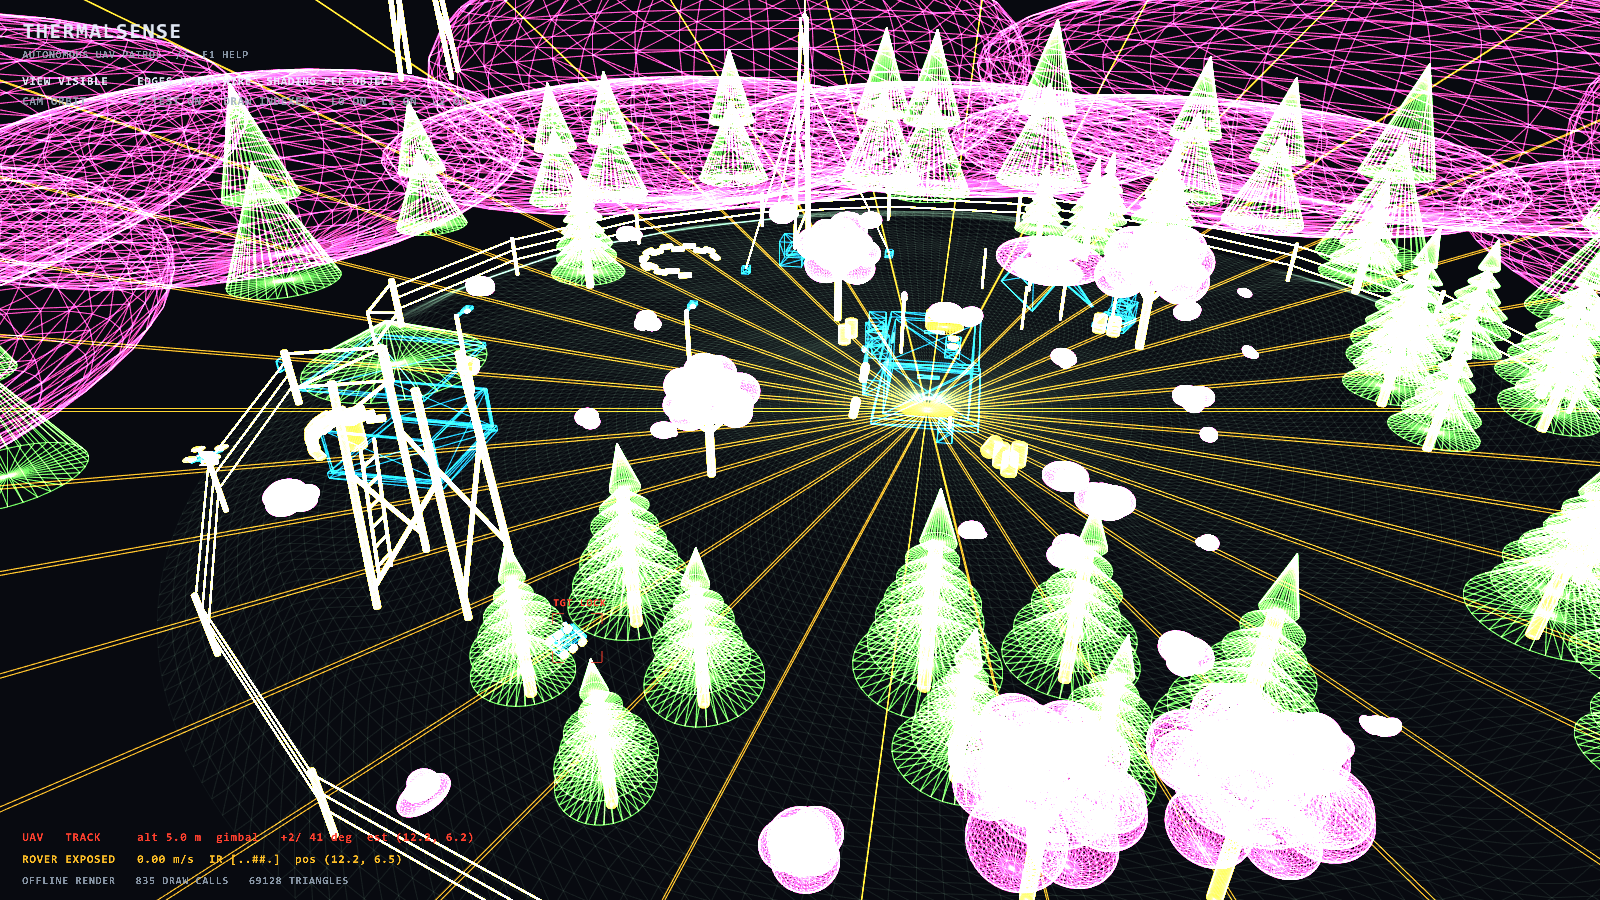
\includegraphics[width=\linewidth]{scene_xray.png}\caption{X-ray edges (by primitive)}\end{subfigure}
  \begin{subfigure}{0.325\linewidth}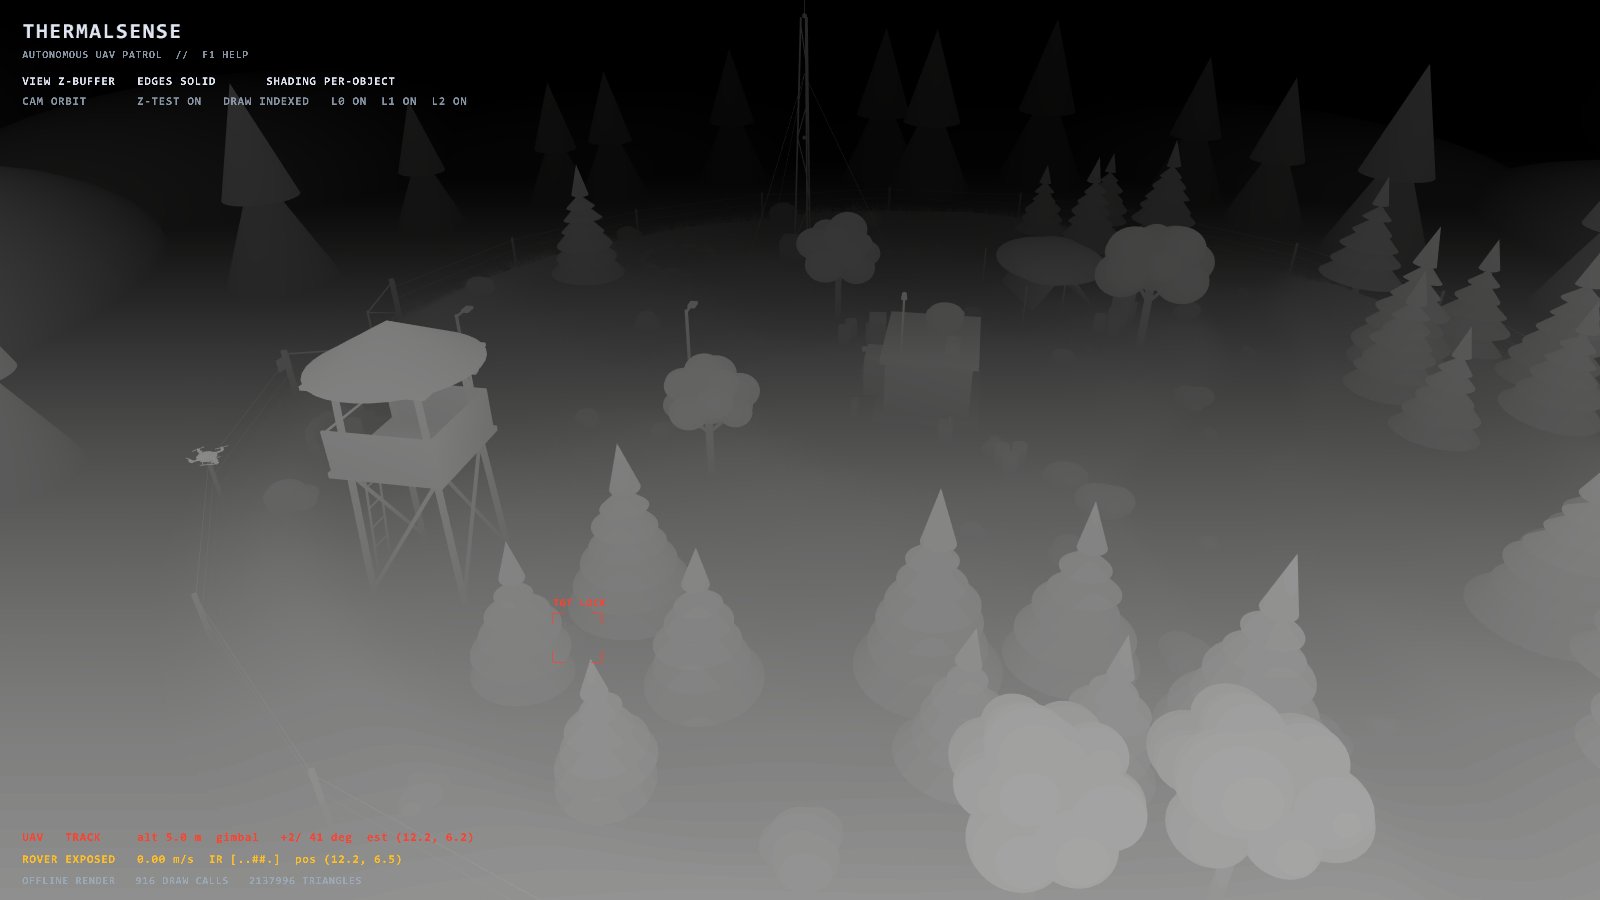
\includegraphics[width=\linewidth]{scene_depth.png}\caption{Z-buffer contents}\end{subfigure}
  \begin{subfigure}{0.325\linewidth}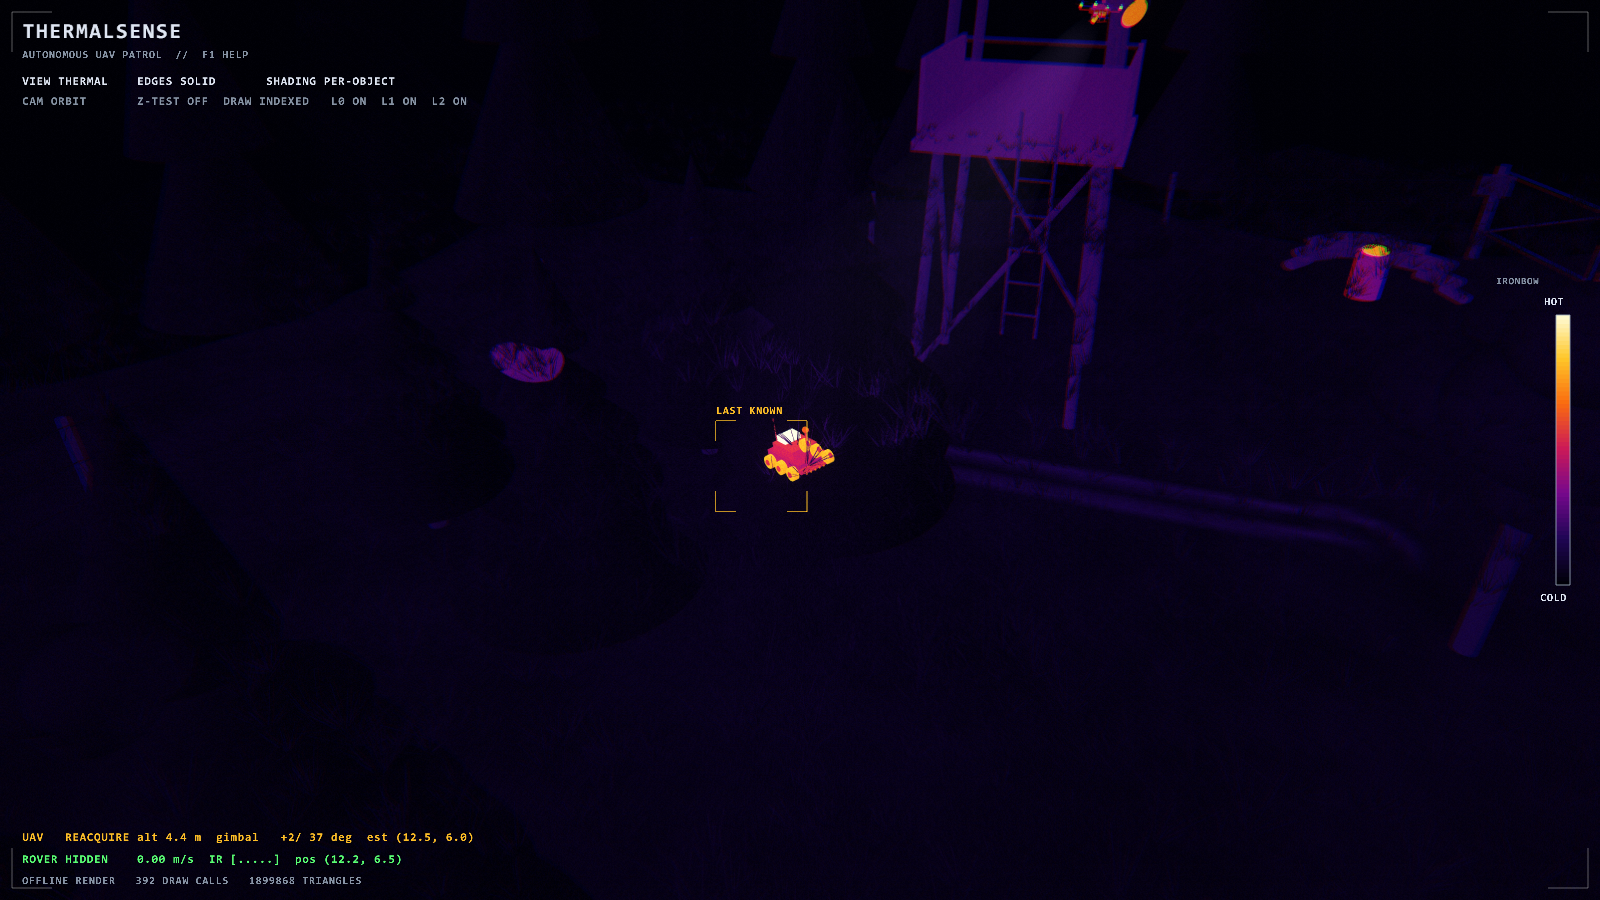
\includegraphics[width=\linewidth]{hide_ztest_off.png}\caption{Depth test off}\end{subfigure}
  \caption{Diagnostic rendering. In (c) the rover, hidden under a spruce in Fig.~\ref{fig:results}c,
  is drawn over the crown because the Z-buffer is disabled.}
  \label{fig:diag}
\end{figure}

% =====================================================================
\section{Autonomous Behaviour}
\textbf{UAV computer vision.} Every frame the scene is rendered from the gimbal camera into a
$320\times240$ off-screen heat image and read back with \texttt{glReadPixels}. Pixels with
$h\ge0.80$ form blobs, and a blob is a target only if it has a core $h\ge0.90$. Blobs are labelled
with an 8-neighbour flood fill ($O(WH)$). The centroid $(u,v)\in[-1,1]^2$ of the chosen blob drives
a visual servo on the gimbal, $\psi_g \leftarrow \psi_g - K\arctan(u\tan\tfrac{\alpha_x}{2})\,\Delta t$
($K=5\,\mathrm{s}^{-1}$), and its ground position is found by marching the pixel ray to the terrain.
The UAV switches between SEARCH (an orbit whose radius swings between 5.5 and 15.5\,m while the camera
sweeps in and out), TRACK and REACQUIRE (circling the last estimate). While tracking it coasts on the
last estimate for 0.75\,s, so brief occlusion by branches does not break the track. It never reads
the rover's true position.

\textbf{Rover: MicroMouse planning + line following.} The disc is split into $80\times80$ cells of
0.5\,m. A cell is a goal if the segments from five body points to the UAV are blocked; each segment
is tested against the exact occluder primitive after mapping it into the primitive's unit space with
$W^{-1}$. A cell is drivable if short vertical segments through the robot's body (centre plus 8
points on its radius, up to mast height 0.8\,m) miss every part, so the robot cannot drive under low
branches or wedge itself between the watchtower's braces. A breadth-first flood fill gives each cell
its step distance $D$ to the nearest goal, and the robot walks downhill ($D\rightarrow D-1$) like a
MicroMouse. The path is smoothed (Chaikin) into a virtual line. Five IR sensors give the error
$e=\overline{x}_\text{active}/0.12$, a PD controller sets $\omega=3.2e+0.25\dot e$, and the
differential drive uses $v_{L,R}=v\mp\omega W/2$; when blocked, the robot pivots and backs off.

% =====================================================================
\section{Results}
Fig.~\ref{fig:results} shows the running system and Table~\ref{tab:measure} the measured values.
Over a 180\,s run the rover drove to new hiding places repeatedly: the UAV was in TRACK 57\,\% of the
time, in REACQUIRE 28\,\% and in SEARCH 14\,\%. It detected the rover in 51\,\% of the samples, and
the rover was hidden in 31\,\%. When detected, the median ground-position error was 0.45\,m (the hot
blob is the motor box, 0.33\,m above the ground). All 49 automated tests and 23 visual checks pass
(Excel sheet \emph{Testing}).

\begin{figure}[h]
  \centering
  \begin{subfigure}{0.495\linewidth}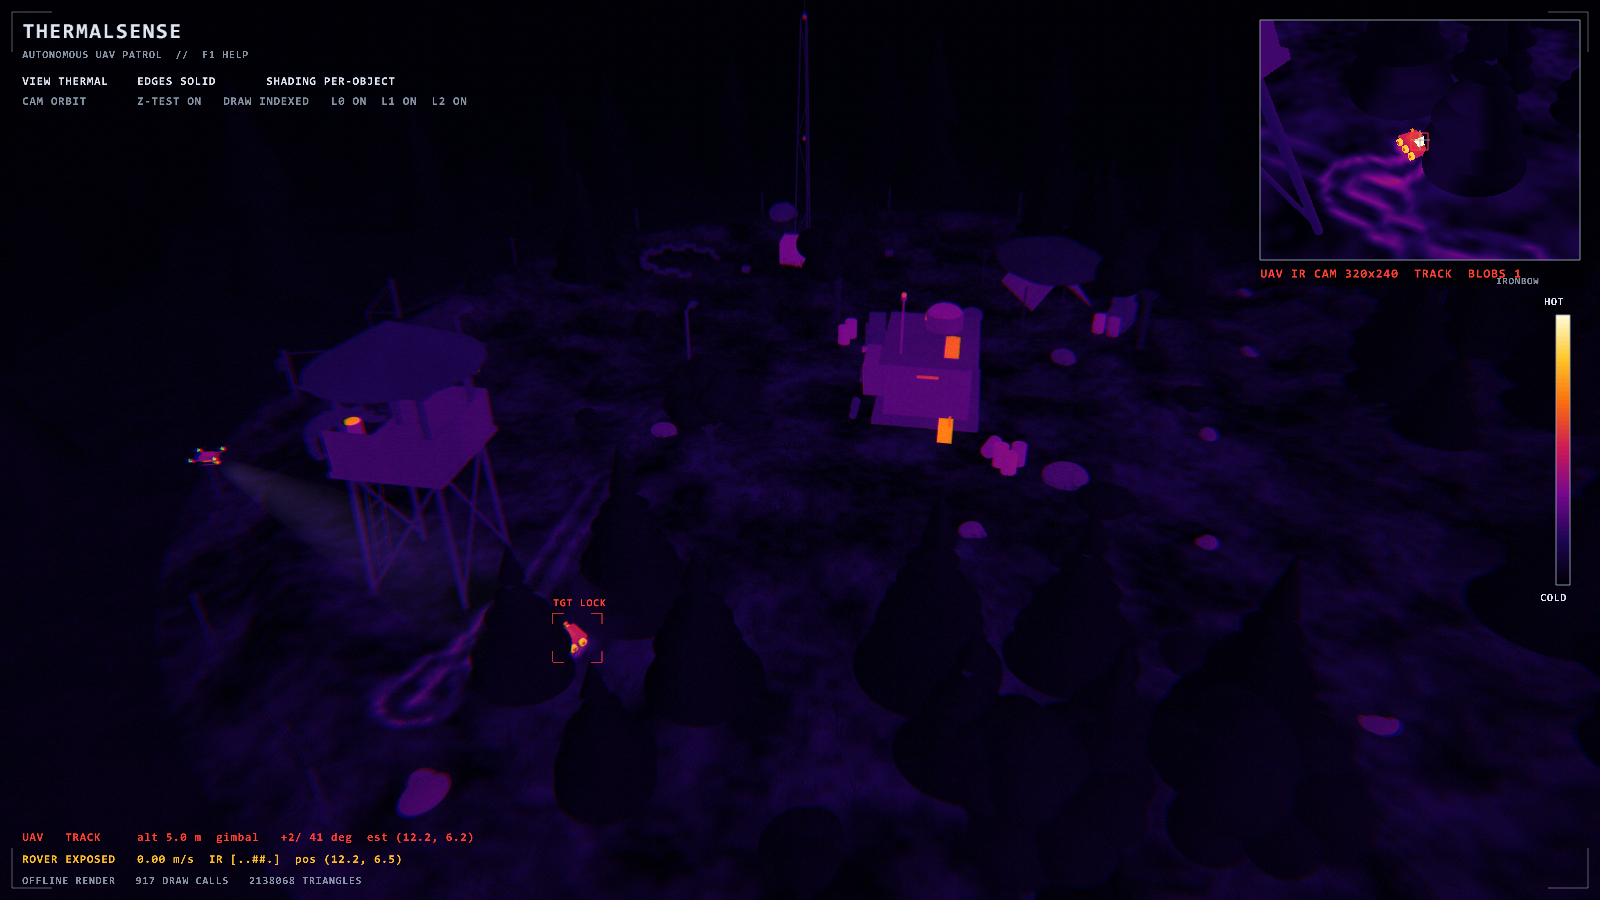
\includegraphics[width=\linewidth]{scene_thermal.png}\caption{Thermal view, UAV tracking (inset: its camera)}\end{subfigure}
  \begin{subfigure}{0.495\linewidth}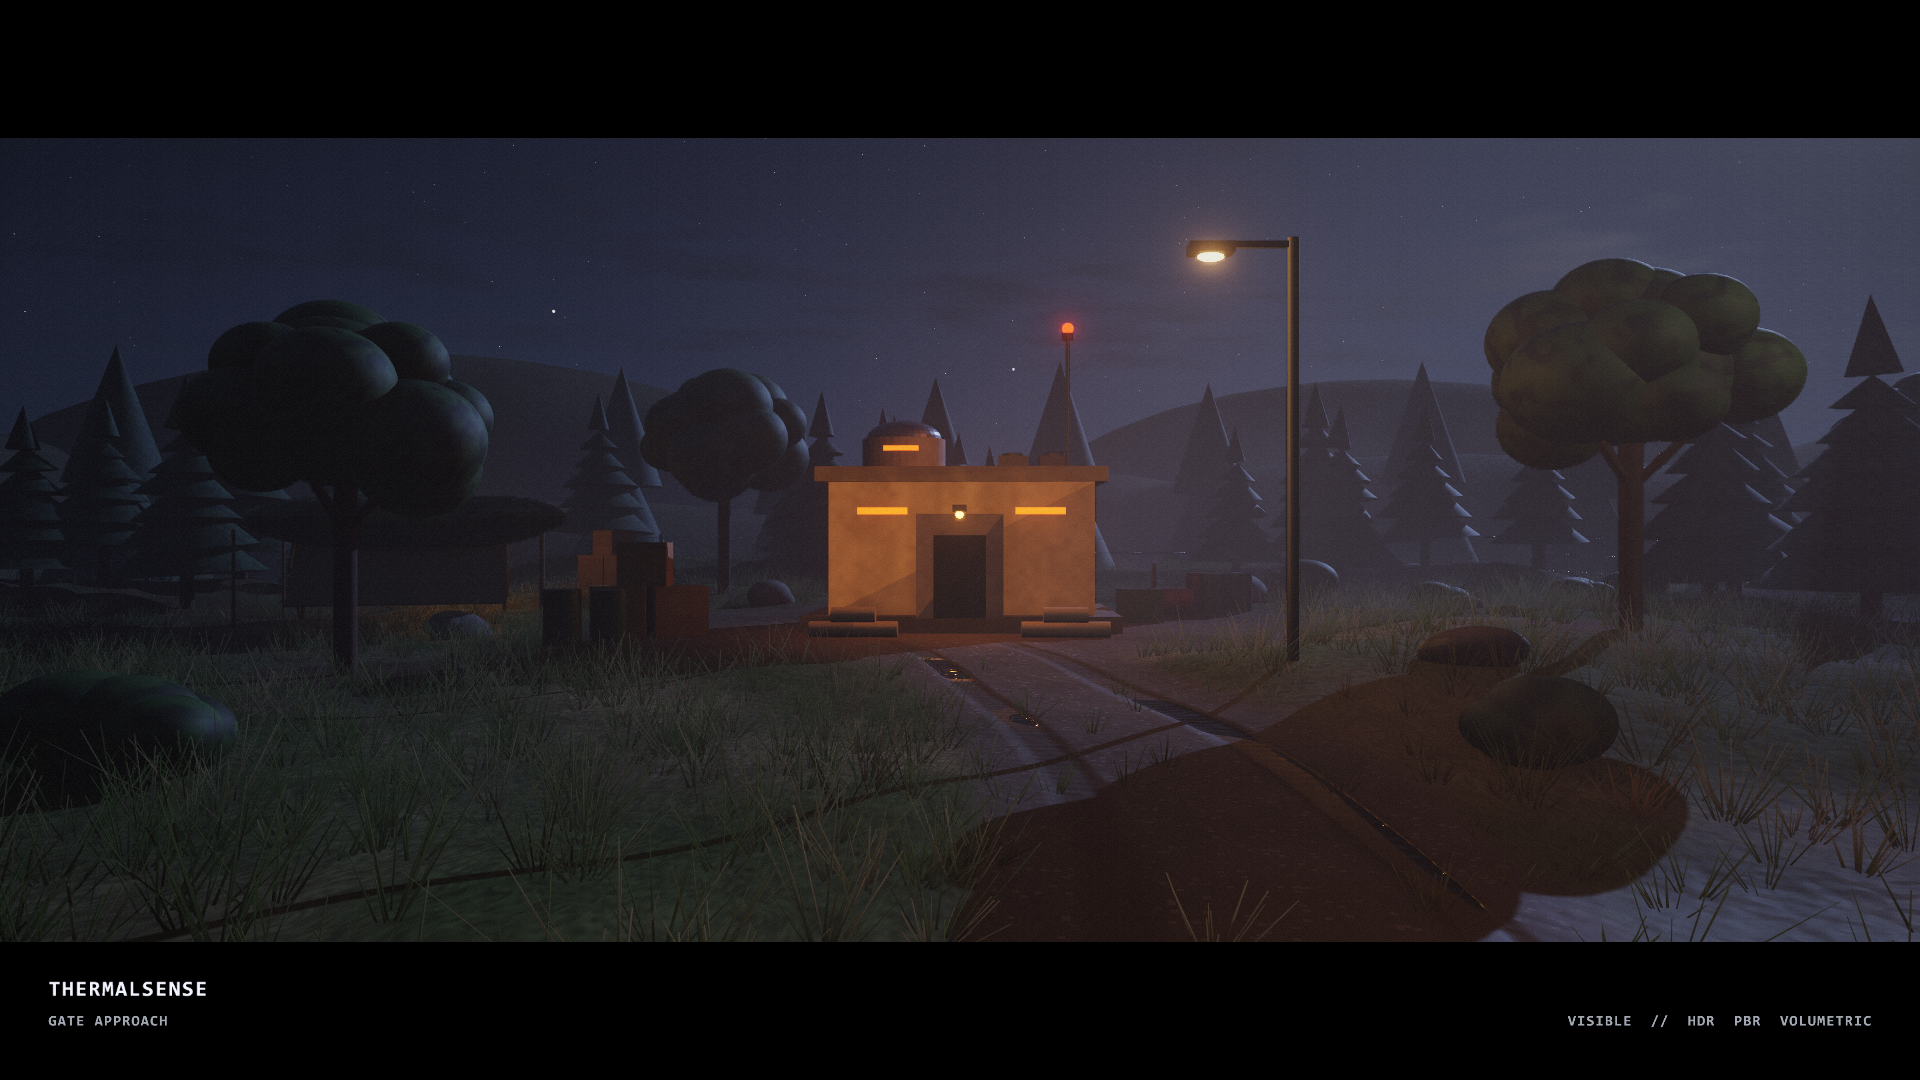
\includegraphics[width=\linewidth]{cine_gate.png}\caption{Ground: turf, grass tufts, tyre ruts, lamps}\end{subfigure}\\[1mm]
  \begin{subfigure}{0.325\linewidth}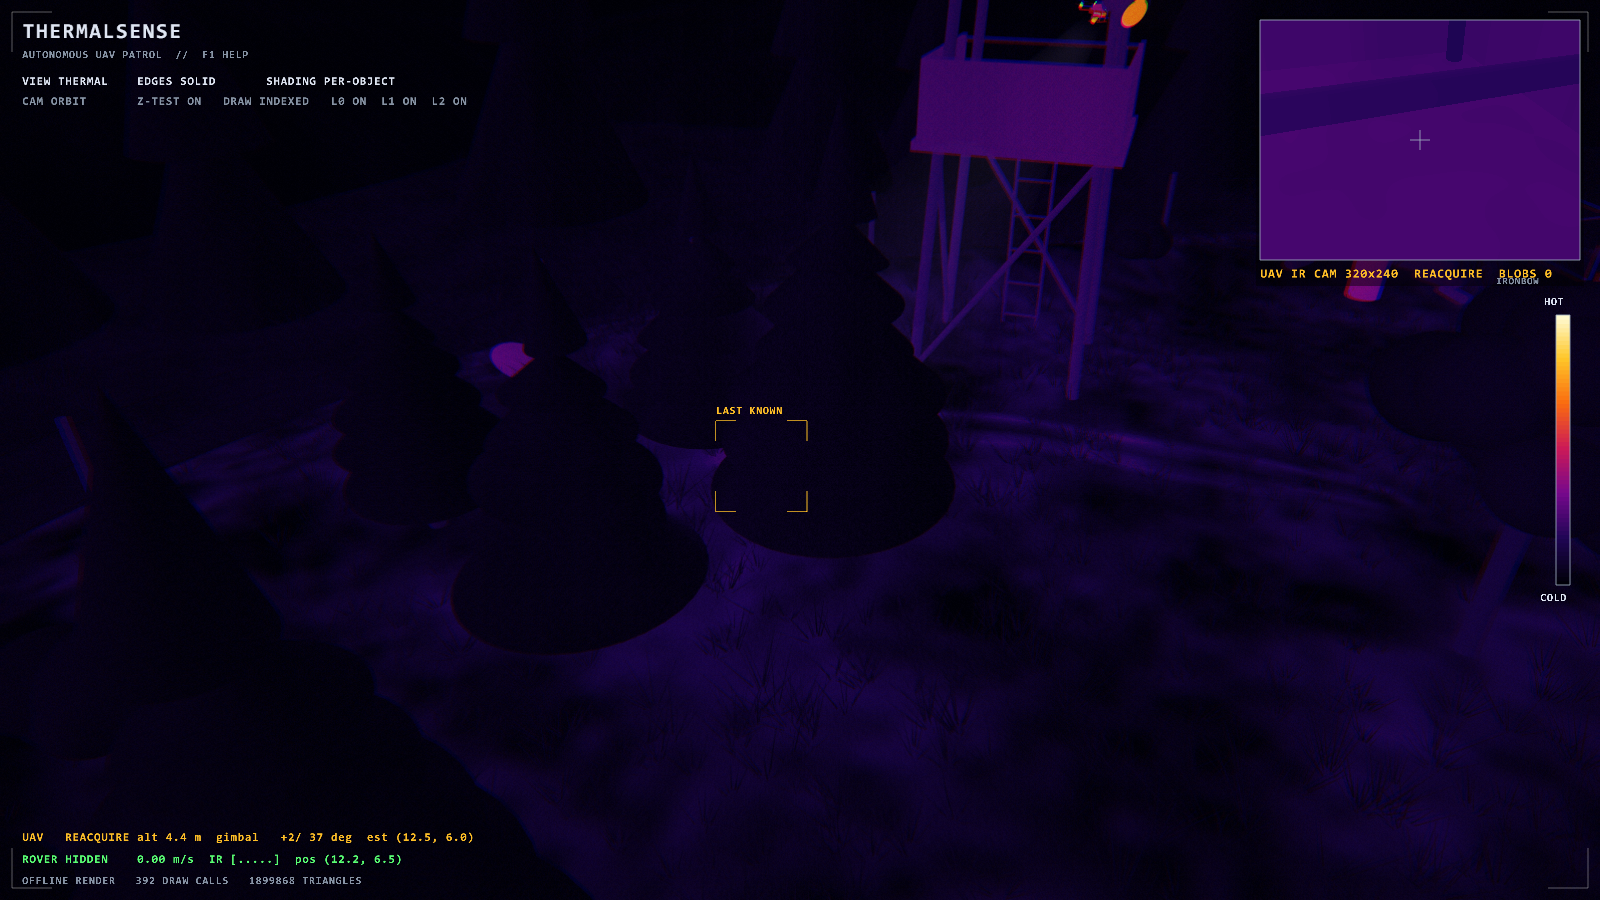
\includegraphics[width=\linewidth]{hide_thermal.png}\caption{Rover hidden, UAV re-acquiring}\end{subfigure}
  \begin{subfigure}{0.325\linewidth}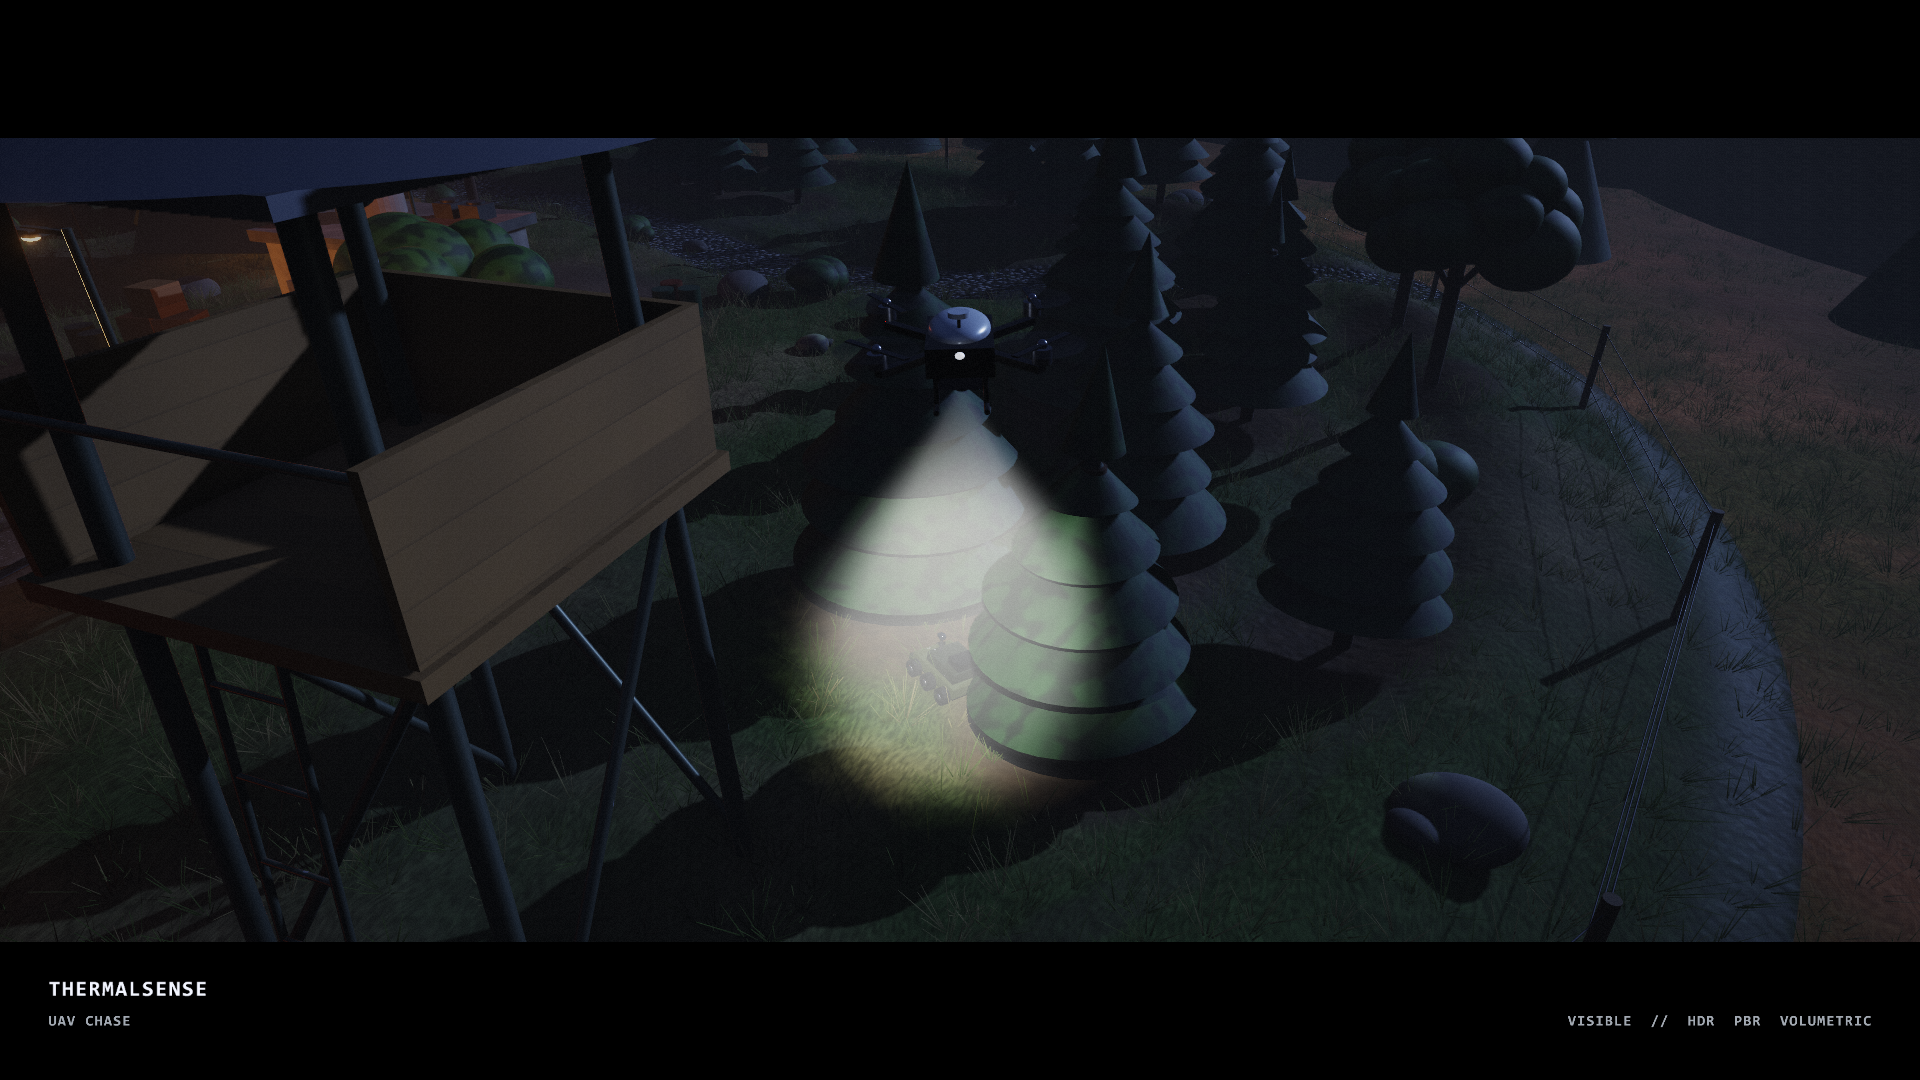
\includegraphics[width=\linewidth]{cine_chase.png}\caption{Volumetric searchlight shaft}\end{subfigure}
  \begin{subfigure}{0.325\linewidth}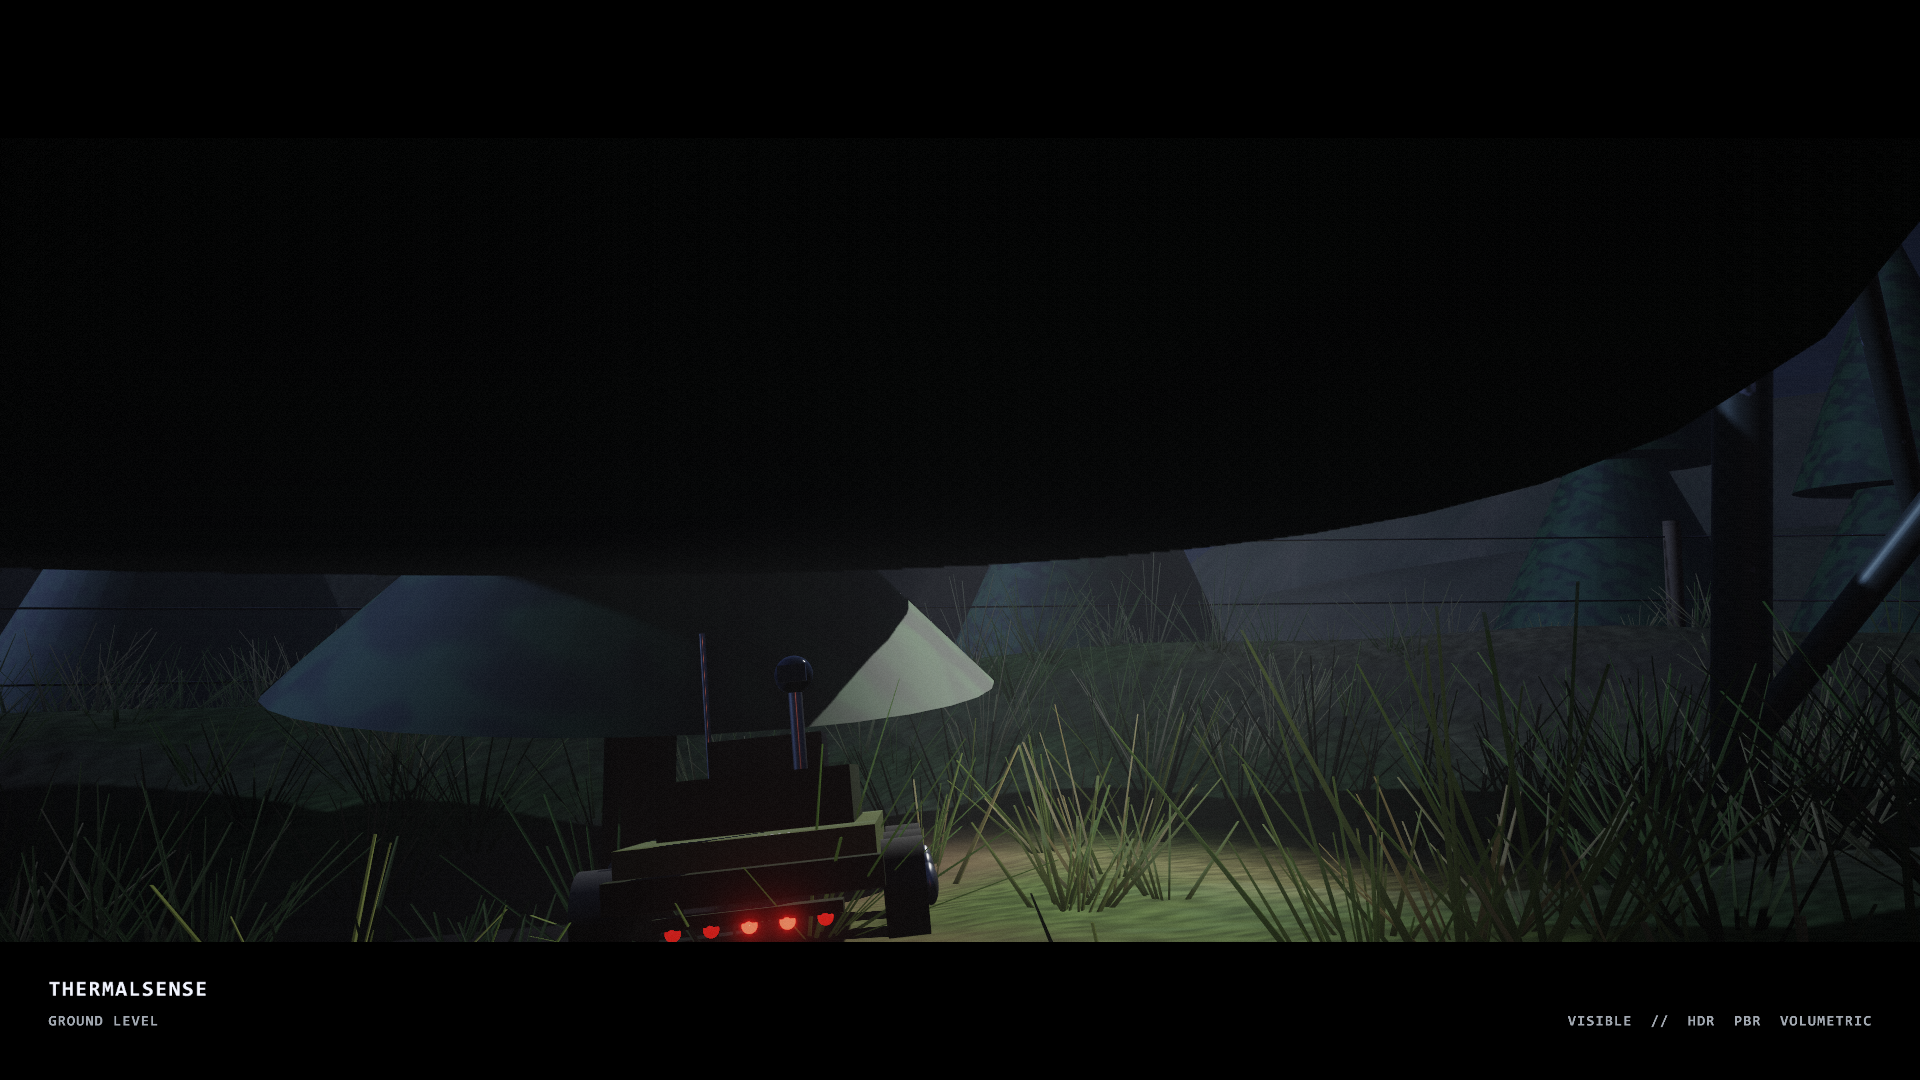
\includegraphics[width=\linewidth]{cine_ground.png}\caption{Ground level: rover and IR sensors}\end{subfigure}
  \caption{ThermalSense results (all images captured from the program with \texttt{-{}-capture}).}
  \label{fig:results}
\end{figure}

\begin{table}[h]
\centering\small
\caption{Measured values (\texttt{-{}-benchmark} at $1280\times720$, High, per-frame averages, and \texttt{-{}-trace 180}); full tables in the Excel workbook.}
\label{tab:measure}
\begin{tabular}{lrr}
\toprule
Quantity & Indexed & Non-indexed\\
\midrule
Frame rate (FPS) / frame time (ms) & 14.7 / 67.9 & 14.3 / 70.1\\
Vertices submitted, main view & 234\,310 & 1\,195\,980\\
Triangles per frame, main view (incl.\ 35\,000 grass blades) & \multicolumn{2}{r}{819\,236}\\
Draw calls per frame: main view / shadow maps / UAV camera & \multicolumn{2}{r}{860 / 203 / 89}\\
\midrule
UAV mode share TRACK / REACQUIRE / SEARCH (180\,s) & \multicolumn{2}{r}{57.2\,\% / 28.4\,\% / 14.5\,\%}\\
Detection share / rover hidden share & \multicolumn{2}{r}{50.9\,\% / 31.2\,\%}\\
Ground-position error when detected (median / p90) & \multicolumn{2}{r}{0.45\,m / 0.67\,m}\\
\bottomrule
\end{tabular}
\end{table}

% =====================================================================
\section{Conclusion}
ThermalSense builds a realistic night-patrol scene from the lab's unit primitives: 805 parts share six
indexed meshes (66\,\% less memory for the sphere and terrain). It covers primitive generation with
CCW winding and normals, VAO/VBO/EBO indexing, instancing, $TRS$ hierarchies, flat/Gouraud/Phong
evaluation of a physically based lighting model, three main lights plus practical lights, shadow
maps, SSAO, volumetric fog, rain with wet surfaces, HDR post-processing, Z-buffering and wireframe
diagnostics, plus a thermal camera with three palettes and heat footprints that cool over time. The same
primitives serve as the geometry for the UAV's thermal vision and for the rover's line-of-sight
planning. The code, the Excel workbook (whose matrices are recomputed and checked by formulas) and
this report all come from the program's own exports and measurements.

\end{document}
